\documentclass[11pt,a4paper]{article}
\usepackage[margin=2.4cm]{geometry}
\usepackage[utf8]{inputenc}
\usepackage{amsmath,amssymb,amsthm,mathtools,bm}
\usepackage{booktabs,array,tabularx,enumitem,float,listings}
\usepackage[dvipsnames]{xcolor}
\usepackage[most]{tcolorbox}
\usepackage{tikz,pgfplots}
\usetikzlibrary{arrows.meta,calc,positioning,shapes.geometric,decorations.pathreplacing,fit,backgrounds,patterns}
\pgfplotsset{compat=1.16}
\usepackage[protrusion=true,expansion=false]{microtype}
\usepackage[colorlinks=true,linkcolor=blue!50!black,citecolor=blue!50!black,urlcolor=blue!50!black]{hyperref}

% ---------- numbering: sections follow the lecture (3.1 ... 3.8) ----------
\renewcommand{\thesection}{3.\arabic{section}}
\numberwithin{equation}{section}
\newcommand{\slides}[1]{\texorpdfstring{\;\emph{(slides #1)}}{ (slides #1)}}

% ---------- macros ----------
\newcommand{\R}{\mathbb{R}}
\newcommand{\E}{\mathbb{E}}
\newcommand{\bx}{\bm{x}}
\newcommand{\bz}{\bm{z}}
\newcommand{\beps}{\bm{\epsilon}}
\newcommand{\K}{\mathbf{K}}
\newcommand{\pv}{\mathbf{p}}
\newcommand{\xt}{\tilde{\mathbf{x}}}
\newcommand{\Rot}{\mathbf{R}}
\newcommand{\tv}{\mathbf{t}}
\newcommand{\AbsRel}{\mathrm{AbsRel}}
\newcommand{\Kinv}{\bm K^{-1}}
\DeclareMathOperator*{\argmin}{arg\,min}
\newcolumntype{Y}{>{\raggedright\arraybackslash}X}

% The lecture reaches section numbers such as 3.10.1, wider than article's
% default table-of-contents number columns.
\makeatletter
\renewcommand*{\l@section}[2]{%
  \ifnum \c@tocdepth >\z@
    \addpenalty\@secpenalty
    \addvspace{1.0em \@plus\p@}%
    \setlength\@tempdima{2.2em}%
    \begingroup
      \parindent \z@ \rightskip \@pnumwidth
      \parfillskip -\@pnumwidth
      \leavevmode \bfseries
      \advance\leftskip\@tempdima
      \hskip -\leftskip
      #1\nobreak\hfil
      \nobreak\hb@xt@\@pnumwidth{\hss #2%
                                 \kern-\p@\kern\p@}\par
    \endgroup
  \fi}
\renewcommand*{\l@subsection}{\@dottedtocline{2}{1.5em}{3.4em}}
\makeatother

% ---------- theorem-like environments in boxes ----------
\theoremstyle{plain}
\newtheorem{theorem}{Theorem}[section]
\newtheorem{proposition}[theorem]{Proposition}
\newtheorem{lemma}[theorem]{Lemma}
\newtheorem{corollary}[theorem]{Corollary}
\theoremstyle{definition}
\newtheorem{definition}[theorem]{Definition}
\newtheorem{example}[theorem]{Example}
\newtheorem{algorithm}[theorem]{Algorithm}
\newtheorem{remark}[theorem]{Remark}

\tcbset{boxenv/.style={enhanced,breakable,boxrule=0.6pt,arc=2pt,left=6pt,right=6pt,top=4pt,bottom=4pt}}
\tcolorboxenvironment{theorem}{boxenv,colback=red!4,colframe=red!55!black}
\tcolorboxenvironment{proposition}{boxenv,colback=orange!5,colframe=orange!75!black}
\tcolorboxenvironment{lemma}{boxenv,colback=orange!5,colframe=orange!75!black}
\tcolorboxenvironment{corollary}{boxenv,colback=orange!5,colframe=orange!75!black}
\tcolorboxenvironment{definition}{boxenv,colback=green!4,colframe=green!45!black}
\tcolorboxenvironment{example}{boxenv,colback=gray!7,colframe=gray!65!black}
\tcolorboxenvironment{algorithm}{boxenv,colback=violet!5,colframe=violet!70!black}
\tcolorboxenvironment{remark}{boxenv,colback=black!3,colframe=black!50}

\newtcolorbox{intuition}{enhanced,breakable,colback=blue!5,colframe=blue!60!black,
  coltitle=white,colbacktitle=blue!60!black,fonttitle=\bfseries,title=Intuition,
  boxrule=0.6pt,arc=2pt,left=6pt,right=6pt,top=4pt,bottom=4pt}

\pgfplotsset{every axis/.append style={width=0.86\linewidth,height=6.2cm,grid=major,
  grid style={gray!25},legend style={font=\small},label style={font=\small},tick label style={font=\small}}}

\lstset{basicstyle=\ttfamily\footnotesize,frame=single,backgroundcolor=\color{gray!6},
  language=Python,keywordstyle=\color{blue!60!black},commentstyle=\color{green!40!black},
  breaklines=true,columns=fullflexible,showstringspaces=false,xleftmargin=4pt,xrightmargin=4pt}

% photo placeholder: \photo[height]{slide}{what to insert}
\newcommand{\photo}[3][2.8cm]{%
  \begin{center}\begin{tikzpicture}
  \node[draw,dashed,thick,fill=gray!8,minimum height=#1,text width=0.8\linewidth,align=center]
    {\textbf{[PHOTO PLACEHOLDER]}\\ Insert the image from \textbf{slide #2}:\\ \emph{#3}};
  \end{tikzpicture}\end{center}}

% image placeholder: {slide}{description}{height}{width}
\newcommand{\phimg}[4]{%
\begin{tikzpicture}
\node[draw=black!50,dashed,fill=black!5,minimum height=#3,minimum width=#4,
      text width=\dimexpr#4-1cm\relax,align=center,inner sep=6pt]
{\textbf{IMAGE PLACEHOLDER}\\[2pt]Insert the picture from \textbf{slide #1}\\[2pt]{\small\itshape #2}};
\end{tikzpicture}}

\tikzset{box/.style={draw,rounded corners=2pt,align=center,minimum height=0.8cm,fill=blue!8,inner sep=3pt,font=\small},
  frozen/.style={box,fill=pink!40},
  arr/.style={-{Stealth[length=2mm]},thick}}

\title{\textbf{Foundations of Spatial AI}\\[4pt]
Lecture 03 --- Single-View Depth\\[4pt]
\large Detailed lecture notes}
\author{Notes based on the slides of L.~Di~Giammarino and E.~Giacomini\\(Sapienza University of Rome, 30 September 2026)}
\date{}

\begin{document}
\maketitle

\begin{tcolorbox}[colback=gray!6,colframe=gray!60,boxrule=0.5pt,arc=2pt]
\textbf{How to read these notes.} Section headers reuse the titles of the slides and are tagged with the slide range they cover. Formal statements (definitions, propositions, theorems, algorithms) are placed where the slides introduce the topic; the slides themselves state most results without proof, so the derivations are added here. Blue \emph{Intuition} boxes explain the ``why'' in plain words, with worked numbers. All figures are original TikZ/pgfplots drawings; figures marked \emph{schematic} show the qualitative trend described on the slides, not measured data.
\end{tcolorbox}

\begingroup
\sloppy
\tableofcontents
\endgroup
\newpage
% =====================================================================
\section{From Image Formation to Measurement \slides{1--3}}
% =====================================================================
Lecture 01 modeled how a scene becomes an image: projection sends a 3D point to a pixel and \emph{discards the distance along the ray}. Lecture 02 covered ways to \emph{represent} a scene: points, meshes, voxels, signed distance functions, Gaussians. Neither lecture covered how to \emph{measure} a scene. This lecture obtains one depth value per pixel (not always -- some sensors leave holes) in one of three ways: by measuring it with a laser, by stereo vision, or by \emph{predicting} it with a learned prior.
 

\begin{figure}[H]
	\centering
	
\includegraphics[width=1.0\linewidth]{1790767754174.png}
\end{figure}

\begin{table}[htbp]
\centering\small
\begin{tabular}{llc}
\toprule
Section & Title & Slides\\
\midrule
3.1 & From representations to measurements & 4--7\\
3.2 & Three ways to pay for depth & 8--12\\
3.3 & Inside a LiDAR & 13--17\\
3.4 & From point cloud to depth image & 18--19\\
3.5 & From recovery to prediction & 20--22\\
3.6 & Cues in closed form & 23--26\\
3.7 & Supervised single-view depth & 27--35\\
3.8 & Cues used by the network & 36--39\\
\bottomrule
\end{tabular}
\caption{The agenda (slide 3) with slide ranges.}
\end{table}
 
\begin{intuition}
The whole lecture is one story: an image is a \emph{projection}, so depth is missing. Every method for getting it back must \emph{pay} with something -- time (a laser pulse), a baseline (a second viewpoint), computation (motion), or a prior (assumptions learned from data). The interesting questions are always: what did we pay, and what is therefore \emph{guaranteed} about the answer?
\end{intuition}
 
% =====================================================================
\section{From Representations to Measurements \slides{4--7}}
% =====================================================================
\emph{What one image determines, and what it does not.} The two preceding lectures modeled image formation and scene representation. This section separates \emph{recovered} from \emph{ambiguous} quantities and shows which of the two depth from one image is.
 
\subsection{Recovered and Ambiguous Quantities \slides{5}}
 
\begin{definition}[Recovered vs.\ ambiguous quantity]
Every quantity estimated in this lecture falls into one of two cases.
\begin{itemize}
\item \textbf{Recovered}: the data determine it up to noise. It can be reported in meters with an error bar.
\item \textbf{Ambiguous}: the data determine it only up to a \emph{family of transformations}. Any single number reported for it comes from an added assumption.
\end{itemize}
\end{definition}
 
\begin{table}[htbp]
\centering\small
\begin{tabular}{lcp{5.6cm}}
\toprule
Quantity & Free parameters & What pins it down\\
\midrule
metric depth & $0$ & nothing, it is already in meters\\
up to scale & $1$ ($s$) & one known length\\
up to scale and shift & $2$ ($s,t$) & two known depths\\
ordering only & any monotone map & a calibrated sensor\\
\bottomrule
\end{tabular}
\caption{Ambiguity ladder (slide 5). The number of free parameters says how much external information is still needed.}
\end{table}
 
\begin{intuition}
Think of the free parameters as \emph{knobs you cannot read from the data}. Metric depth has no knob. ``Up to scale'' has one knob: the scene may be uniformly inflated or shrunk. ``Up to scale and shift'' has two. ``Ordering only'' is the weakest: you know that $A$ is nearer than $B$, but $(1,2,3)$ and $(1,10,100)$ tell exactly the same story. The slide's punchline: disagreements about depth estimation are usually disagreements about \emph{which row of this table a quantity lives in}.
\end{intuition}
 
\subsection{The Back-Projected Ray \slides{6}}
 
Projection throws one number away per pixel; inverting it asks for that number back:
\begin{equation}\label{eq:backproj}
\bm p^{c} \;=\; z\,\Kinv\,\xt_s .
\end{equation}
Here $\xt_s$ is the homogeneous pixel (third component $1$), $\bm K$ the intrinsics from lecture 01, and $\bm p^c$ the point in the camera frame.
 
\begin{proposition}[Projection is not invertible]\label{prop:ray}
The third component of $\Kinv\xt_s$ is $1$, so the free scalar $z$ in \eqref{eq:backproj} is the depth in meters along the optical axis. Given only $\bm x_s$, the set of 3D points that project to it is the whole ray
\[
\{\, z\,\Kinv\xt_s \;:\; z>0 \,\}.
\]
\end{proposition}
\begin{proof}
Third row of $\bm K$ is $(0,0,1)$, hence $\bm K\bm p^c=(\ast,\ast,p^c_z)^\top$ and $\bm p^c$ projects to $\xt_s$ iff $\bm K\bm p^c=\lambda\xt_s$ with $\lambda=p^c_z$ (homogeneous division). Solving, $\bm p^c=\lambda\Kinv\xt_s$ and $\lambda=z$. Conversely every $z\Kinv\xt_s$ satisfies $\bm K(z\Kinv\xt_s)=z\xt_s\sim\xt_s$. \qedhere
\end{proof}
 
\begin{figure}[htbp]
\centering
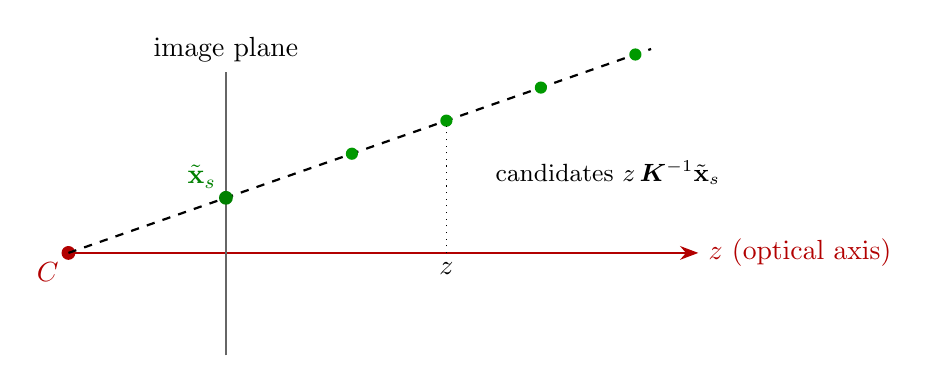
\begin{tikzpicture}[>=Stealth]
\draw[->,thick,red!70!black] (0,0)--(8,0) node[right]{$z$ (optical axis)};
\draw[thick,black!60] (2,-1.3)--(2,2.3) node[above,black]{image plane};
\fill[red!70!black] (0,0) circle(2.5pt) node[below left]{$C$};
\draw[dashed,thick] (0,0)--(7.4,2.59);
\fill[green!50!black] (2,0.7) circle(2.5pt) node[above left]{$\xt_s$};
\foreach \zz in {3.6,4.8,6.0,7.2} \fill[green!60!black] (\zz,{0.35*\zz}) circle(2.2pt);
\draw[dotted] (4.8,0)--(4.8,1.68);
\node[below] at (4.8,0) {$z$};
\node[anchor=north west] at (5.3,1.3) {\small candidates $z\,\Kinv\xt_s$};
\end{tikzpicture}
\caption{Back-projected ray (redrawn from slide 6; side view, $y$ up). Every green point projects to the same pixel.}\label{fig:ray}
\end{figure}
 
\begin{intuition}
It is like knowing the \emph{direction} in which a laser pointer is aimed but not how far away the dot lands. The information was \emph{destroyed at capture}, not merely hidden: no clever algorithm can un-destroy it, so every method that produces $z$ is either measuring something extra or importing an assumption. ``Producing $z$ at every pixel is the whole of this lecture.''
\end{intuition}
 
\subsection{Scale-Depth Ambiguity \slides{7}}
 
\begin{proposition}[Global scale is unobservable from one image]\label{prop:scale}
Let $\{\bm p_j\}$ be a scene in the camera frame and $s>0$. The scaled scene $\{s\bm p_j\}$ produces exactly the same image.
\end{proposition}
\begin{proof}
$\pi(\bm K\,s\bm p)=\pi(s\,\bm K\bm p)=\pi(\bm K\bm p)$, because the homogeneous division cancels $s$. \qedhere
\end{proof}
 
\begin{figure}[htbp]
\centering
\begin{tikzpicture}[>=Stealth]
\fill[blue!60!black] (0,0) circle(2pt) node[left]{eye};
\draw[dashed,blue!60!black] (0,0)--(8,1.6);
\draw[dashed,blue!60!black] (0,0)--(8,-1.6);
\draw[thick,black!60] (1.5,-0.3)--(1.5,0.3) node[above]{\scriptsize image};
\draw[very thick,red!70!black] (3,-0.6)--(3,0.6) node[above]{\scriptsize small, near};
\draw[very thick,red!70!black] (6,-1.2)--(6,1.2) node[above]{\scriptsize large, far};
\end{tikzpicture}
\caption{Scale-depth ambiguity (schematic after slide 7): a small near object and an object twice as large at twice the distance subtend the same angle.}
\end{figure}
 
\begin{figure}[H]
	\centering
	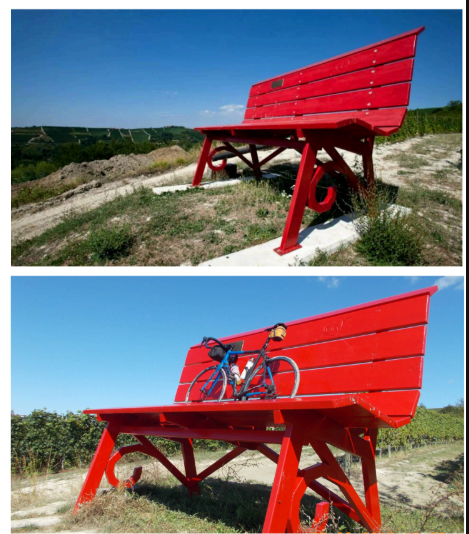
\includegraphics[width=1.0\linewidth]{1790767924564.png}
	\caption{two photos of a giant red bench, the second with a bicycle placed on it}\label{fig:1790767924564}
\end{figure}
 
\begin{intuition}
A small close object looks the same as a much larger one further away. The giant bench in the slide's photographs is a real-life example: on its own it reads as a normal bench, and only the bicycle on top reveals its true size. That bicycle is exactly a \emph{prior about sizes} -- the theme of the rest of the lecture.
\end{intuition}
 
% =====================================================================
\section{Three Ways to Pay for Depth \slides{8--12}}
% =====================================================================
\emph{Time, a baseline, a prior.} No method returns depth for free. Each buys it with a different resource, and the resource decides what the result is good for.
 
\subsection{Two Measurement Principles \slides{9}}
 
\begin{definition}[Time of flight and triangulation]
Two independent choices: the \emph{principle} decides what is measured; the \emph{illumination} decides only whether the sensor brings its own light (\emph{active}) or uses ambient light (\emph{passive}).
\begin{itemize}
\item \textbf{Time of flight (ToF)}: measure the delay of emitted light.
\item \textbf{Triangulation}: measure the angular/pixel difference between two viewpoints separated by a known geometry.
\end{itemize}
\end{definition}
 
\begin{table}[htbp]
\centering\small
\sloppy
\hbadness=10000
\begin{tabularx}{\linewidth}{@{}p{3.1cm}YY@{}}
\toprule
 & time of flight & triangulation\\
\midrule
\textbf{active} (own light) & scanning laser, flash range camera & projected-pattern camera, active stereo\\
\textbf{passive} (ambient light) & \emph{empty}: timing needs a known emission & stereo with a known baseline, structure from motion\\
\bottomrule
\end{tabularx}
\caption{The two-by-two of depth sensing (slide 9).}
\end{table}
 
 
\begin{figure}[H]
	\centering
	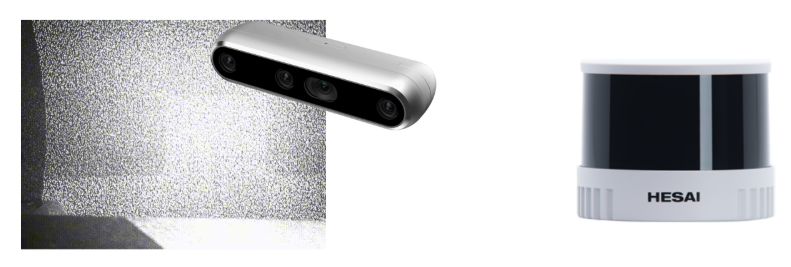
\includegraphics[width=1.0\linewidth]{1790767988279.png}
	\caption{left: speckle pattern of a projected-pattern camera with a stereo camera overlaid; right: a Hesai spinning LiDAR}\label{fig:1790767988279}
\end{figure}

\begin{intuition}
The empty cell is instructive: to time light you must \emph{know when it left}, and ambient light has no known departure time. Also, ``active'' only helps with texture or timing -- it does not change the physics: a projected pattern camera is still triangulation, it just paints texture onto blank walls so matching works.
\end{intuition}
 
\subsection{Triangulation From Two Views \slides{10}}
 
Two rectified cameras sit a baseline $b$ apart. A scene point $\bm p=(x,y,z)\in\R^3$ appears at horizontal pixel offsets $u_L$ and $u_R$ (relative to each principal point), and similar triangles give the depth.
 
\begin{theorem}[Depth from disparity]\label{thm:stereo}
For two rectified cameras with focal length $f$ (in pixels) and baseline $b$ (in meters), the depth of a point with disparity $d=u_L-u_R$ is
\[
z=\frac{f\,b}{d}.
\]
\end{theorem}
\begin{proof}
By the pinhole model $u_L=f\,x/z$ for the left camera, and since the right camera is displaced by $b$ along $x$, $u_R=f\,(x-b)/z$. Subtracting, $d=u_L-u_R=fb/z$. (The slide draws the image plane behind the pinhole, which produces the minus signs in its two similar-triangle equations; the resulting formula is the same.) \qedhere
\end{proof}
 
\begin{figure}[htbp]
\centering
\begin{tikzpicture}[>=Stealth,scale=1.1]
\fill (0,0) circle(2pt) node[below]{$C_L$};
\fill (3,0) circle(2pt) node[below]{$C_R$};
\draw[<->,orange!80!black] (0,-0.6)--(3,-0.6) node[midway,below]{$b$};
\draw[thick,black!60] (-0.9,1)--(0.9,1);
\draw[thick,black!60] (2.1,1)--(3.9,1);
\draw[dashed,gray] (0,0)--(0,1.5);
\draw[dashed,gray] (3,0)--(3,1.5);
\fill[blue!60!black] (1.6,4) circle(2.5pt) node[above]{$\bm p=(x,y,z)$};
\draw (0,0)--(1.6,4);
\draw (3,0)--(1.6,4);
\fill[red!70!black] (0.4,1) circle(1.8pt);
\fill[red!70!black] (2.65,1) circle(1.8pt);
\node[red!70!black,above] at (0.2,1.02) {\scriptsize $u_L$};
\node[red!70!black,above] at (2.82,1.02) {\scriptsize $u_R$};
\draw[<->] (-1.3,0)--(-1.3,1) node[midway,left]{$f$};
\draw[<->,gray] (4.4,0)--(4.4,4) node[midway,right]{$z$};
\end{tikzpicture}
\caption{Rectified stereo (redrawn from slide 10, top view). With $f=1$, $b=3$, $z=4$ as drawn: $u_L=0.4$, $u_R=-0.35$, $d=0.75=fb/z$.}
\end{figure}
 
\begin{corollary}[Unknown baseline]\label{cor:unknownb}
Disparity is inverse depth scaled by $fb$: $1/z=d/(fb)$. If $b$ is unknown (a moving camera), depth is known only up to one global scale.
\end{corollary}
 
\begin{example}
For $f=700$\,px and $b=0.5$\,m, $fb=350$ px\,m and $z=350/d$: $d=70$\,px means $5$\,m, $d=17.5$\,px means $20$\,m, $d=7$\,px means $50$\,m.
\end{example}
 
\begin{intuition}
\textbf{Where meters come from:} $b$ is in meters, so $z$ is in meters -- the baseline is the source of scale. Hold a finger at arm's length and blink one eye at a time: the finger jumps a lot against the background; a distant tree barely moves. That jump \emph{is} the disparity, and it is large for near things (large $1/z$). \textbf{Matching} is the price: $d$ requires finding the \emph{same} point in both images, which fails on textureless or repetitive surfaces and wherever a surface is visible to one view only. Because disparity is $fb$ times inverse depth, an unknown rig only leaves an unknown \emph{scale} in disparity, which is why affine invariance in \emph{disparity} suits data whose rig is unknown (used in \S3.7).
\end{intuition}
 
\subsection{The Three Currencies \slides{11}}
 
\begin{table}[htbp]
\centering\small
\begin{tabularx}{\linewidth}{@{}p{2.2cm}YYY@{}}
\toprule
pay with & method & gives & costs\\
\midrule
\textbf{time} & emit a pulse and time the return (LiDAR) & metric depth, directly & sparse, expensive, returns missing\\
\textbf{a baseline} & stereo, baseline known & metric depth, dense where matching works & a calibrated second camera; error growing as $z^2$\\
\textbf{computation} & structure from motion, baseline unknown & shape up to one global scale & a moving camera and a rigid scene\\
\textbf{a prior} & assumptions learned from data & dense, from one image, cheap & not metric, and only as good as the prior\\
\bottomrule
\end{tabularx}
\caption{The three currencies (slide 11).}
\end{table}
 
\subsection{The Single-Image Claim \slides{12}}
 
The usual motivation for single-image depth is that it bypasses \emph{all} these limitations. The slide's verdict: a single image does bypass the \textbf{cost}, the \textbf{sparsity} and the \textbf{hardware}, but it cannot bypass the \textbf{physics}, because it \emph{never measured anything}. The result is therefore an \emph{ambiguous} quantity (same ray picture as Figure~\ref{fig:ray}).
 
\begin{intuition}
Single-image depth is not a cheaper LiDAR; it is a different kind of object. It converts the question ``how far?'' into ``how far, \emph{given how scenes usually look}?'' -- a guess with an informed prior. Keeping this distinction in mind explains every failure mode in \S3.8.
\end{intuition}
 
% =====================================================================
\section{Inside a LiDAR \slides{13--17}}
% =====================================================================
\emph{Paying with time.} Outdoor depth labels are produced by a scanning laser, and their error sources are inherited by any network trained on them -- so we need to know how a LiDAR fails.
 
\subsection{Pulsed Time of Flight \slides{14}}
 
A short pulse is emitted and a clock runs until the echo returns. The light covers the distance twice, so the interval is halved:
\begin{equation}\label{eq:tof}
r=\frac{c\,t}{2}.
\end{equation}
Each beam leaves in a known direction, so a return is a \emph{direction plus a range}; the energy that comes back is reported as \emph{intensity}. Pulse widths are a few nanoseconds (typically 5--10\,ns, about 4\,ns in modern full-waveform scanners). Every other part of the sensor exists to make the interval $t$ reliable.
 
\begin{example}
An echo from $50$\,m returns after $t=2\cdot 50/(3\cdot10^8)\approx 333$\,ns. A timing error of $1$\,ns corresponds to $c\,\delta t/2\approx 15$\,cm of range. A $5$\,ns pulse is $c\cdot 5\,\text{ns}\approx1.5$\,m long in space.
\end{example}
 
\begin{intuition}
It is echolocation with light: shout and time the echo. The factor $\tfrac12$ is just the round trip. Because $c$ is so large, centimeter accuracy demands sub-nanosecond timing -- which is why timing electronics dominate the design.
\end{intuition}
 
\subsection{Structured Sparsity \slides{15}}
 
Azimuth resolution is set by the spin rate; elevation resolution is fixed in hardware. The two differ, so the sampling is \emph{anisotropic}.
 
\begin{definition}[Scan-line spacing]
For a vertical angular pitch $\Delta\theta_{\text{el}}$ (radians), the spacing between adjacent scan lines at range $r$ is
\[
s(r)\approx r\,\Delta\theta_{\text{el}}.
\]
\end{definition}
 
\begin{example}[Velodyne VLP-16]
At $5$\,Hz the sensor samples every $0.1^\circ$ in azimuth; at $20$\,Hz every $0.4^\circ$ -- spinning faster costs horizontal resolution. Vertically it is stuck at $\Delta\theta_{\text{el}}=2.0^\circ=0.0349$\,rad, so the scan lines are $0.70$\,m apart at $20$\,m and $1.75$\,m apart at $50$\,m. A pedestrian at $50$\,m is crossed by one scan line or by none. (For comparison, the azimuth gap at $50$\,m is only $0.09$\,m at $5$\,Hz and $0.35$\,m at $20$\,Hz.)
\end{example}
 
\begin{figure}[htbp]
\centering
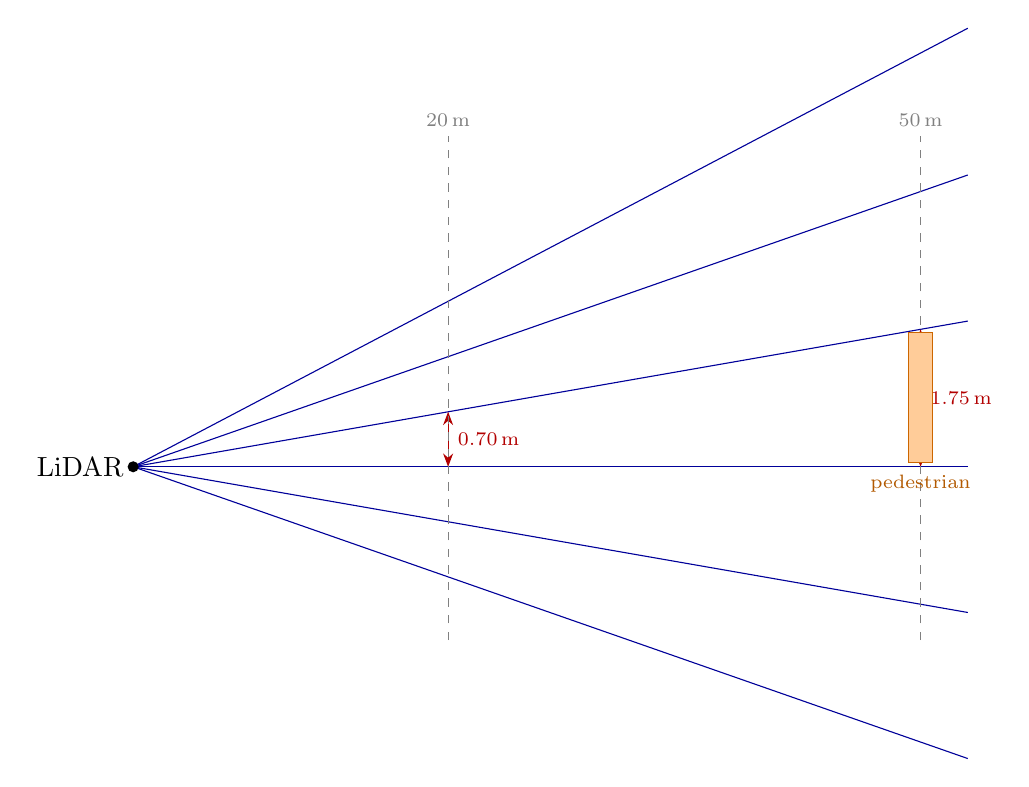
\begin{tikzpicture}[>=Stealth,x=1cm,y=1cm]
% horizontal: 1 cm = 5 m ; vertical: 1 cm = 1 m  (exaggerated vertically)
\foreach \k in {-2,-1,0,1,2,3}{
  \draw[blue!60!black] (0,0)--(10.6,{5*tan(2*\k)*10.6});
}
\fill (0,0) circle(2pt) node[left]{LiDAR};
\draw[<->,red!70!black] (4,0)--(4,{5*tan(2)*4}) node[midway,right]{\scriptsize $0.70$\,m};
\draw[<->,red!70!black] (10,0)--(10,{5*tan(2)*10}) node[midway,right]{\scriptsize $1.75$\,m};
\draw[dashed,gray] (4,-2.2)--(4,4.2) node[above]{\scriptsize $20$\,m};
\draw[dashed,gray] (10,-2.2)--(10,4.2) node[above]{\scriptsize $50$\,m};
% pedestrian, 1.7 m tall, between two rays at 50 m
\draw[fill=orange!40,draw=orange!80!black] (9.85,0.06) rectangle (10.15,1.70);
\node[orange!70!black,below] at (10,0.02) {\scriptsize pedestrian};
\end{tikzpicture}
\caption{Original figure (not on the slides): VLP-16 elevation fan with a $2^\circ$ pitch, side view. Vertical axis exaggerated: $1$\,cm~=~$1$\,m vertically but $1$\,cm~=~$5$\,m along range. At $50$\,m a $1.7$\,m pedestrian fits between two consecutive scan lines and is missed.}
\end{figure}
 

\begin{figure}[H]
	\centering
	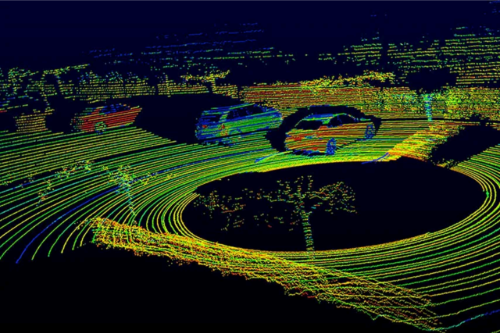
\includegraphics[width=1.0\linewidth]{1790768067024.png}
	\caption{colored LiDAR point cloud of a parking lot: concentric ring-like scan lines with gaps between them}\label{fig:1790768067024}
\end{figure}
 
\begin{intuition}
Picture the grooves of a vinyl record. Samples are dense \emph{along} a groove (azimuth) but grooves are far apart (elevation). Moving away from the sensor, the grooves spread linearly with range, while points along a groove stay comparatively tight. So a point cloud thins with distance along \emph{one axis} much faster than the other, and the gaps form horizontal stripes.
\end{intuition}
 
\subsection{Limitations of a LiDAR Point Cloud \slides{16}}
 
\begin{itemize}
\item \textbf{No color and no semantics.}
\item \textbf{No measurement where there was no return}, which is \emph{distinct from a zero depth}: ``I saw nothing'' is not ``the surface is at distance $0$''.
\item \textbf{No sample between scan lines}, and that gap grows linearly with range.
\item \textbf{Points that lie on no surface}: where one pulse straddles a silhouette, the echo mixes foreground and background into a single (wrong) range.
\end{itemize}
 
\begin{intuition}
The last item is the LiDAR analogue of an out-of-focus edge: half the beam hits the near object, half the far wall, and the reported range is somewhere in the empty air between them. Such ``flying'' points are a systematic error that a network trained on LiDAR labels will inherit at every object boundary.
\end{intuition}
 
\subsection{Two Error Laws \slides{17}}
 
The two principles fail in different ways, and the difference decides where each is worth using.
\[
\text{time of flight: }\ \delta r=\frac{c\,\delta t}{2},
\qquad
\text{triangulation: }\ \delta z\approx\frac{z^{2}\,\delta d}{f\,b}.
\]
 
\begin{proposition}[Triangulation error law]\label{prop:errlaw}
A disparity error $\delta d$ produces a depth error $\delta z\approx z^2\delta d/(fb)$: quadratic in range, even for a perfect sensor.
\end{proposition}
\begin{proof}
From Theorem~\ref{thm:stereo}, $z=fb/d$, so $\left|\frac{dz}{dd}\right|=\frac{fb}{d^2}=\frac{z^2}{fb}$. Multiply by $\delta d$. \qedhere
\end{proof}
 
The timing floor $c\,\delta t/2$ is \emph{independent of range}. What degrades with range is the \emph{precision}: the returned power falls as $1/r^2$ or $1/r^4$ (depending on whether the target is extended or smaller than the beam -- standard radar/LiDAR-equation background), and a weaker return is timed less precisely.
 
\begin{example}[Numbers from the slide]
With $f=700$\,px, $b=0.5$\,m and quarter-pixel matching ($\delta d=0.25$\,px), $fb=350$ and
\[
\delta z(5\,\text{m})=\tfrac{25\cdot0.25}{350}\approx 2\,\text{cm},\quad
\delta z(20\,\text{m})\approx 29\,\text{cm},\quad
\delta z(50\,\text{m})\approx 1.8\,\text{m}.
\]
The laser is exact where it lands, but at $50$\,m its scan lines are $1.75$\,m apart, so a pedestrian is crossed at most once.
\end{example}
 
\begin{figure}[htbp]
\centering
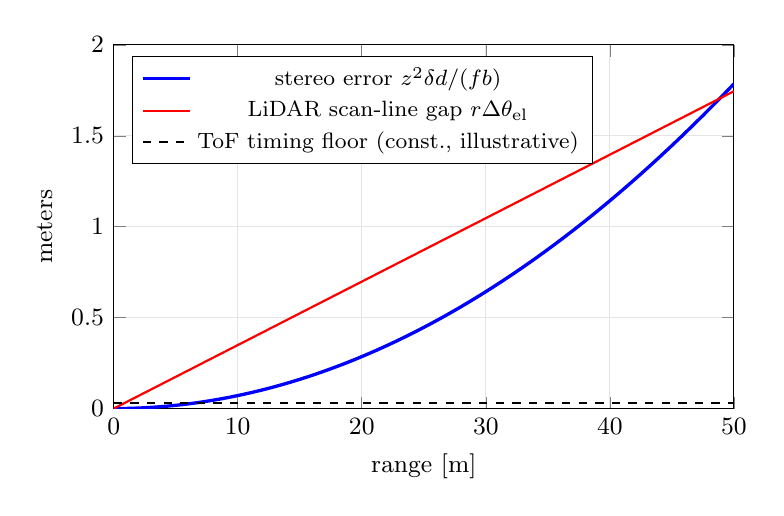
\begin{tikzpicture}
\begin{axis}[width=0.78\linewidth,height=6.2cm,xlabel={range [m]},ylabel={meters},xmin=0,xmax=50,ymin=0,ymax=2,
  legend style={at={(0.03,0.97)},anchor=north west,font=\footnotesize},grid=both,grid style={gray!20}]
\addplot[blue,very thick,domain=0:50,samples=60]{x^2*0.25/350};
\addlegendentry{stereo error $z^2\delta d/(fb)$}
\addplot[red,thick,domain=0:50,samples=2]{0.0349066*x};
\addlegendentry{LiDAR scan-line gap $r\Delta\theta_{\mathrm{el}}$}
\addplot[black,dashed,thick,domain=0:50,samples=2]{0.03};
\addlegendentry{ToF timing floor (const., illustrative)}
\end{axis}
\end{tikzpicture}
\caption{Original figure (not on the slides), from the slide's numbers: $f=700$\,px, $b=0.5$\,m, $\delta d=0.25$\,px, $\Delta\theta_{\text{el}}=2^\circ$. The ToF floor level ($3$\,cm) is only illustrative.}
\end{figure}
 
\begin{intuition}
The two sensors are \emph{complementary}: LiDAR is precise where it samples but leaves holes; stereo samples everywhere but each sample degrades quadratically. This is why the remaining sections either \emph{fuse} the two or \emph{replace the laser with a prior}.
\end{intuition}
 
% =====================================================================
\section{From Point Cloud to Depth Image \slides{18--19}}
% =====================================================================
\emph{Paying with time: from cloud to depth map.} A LiDAR produces a point cloud. Converting it to a depth map needs the extrinsic calibration, the intrinsics (lecture 01), and a rule for resolving points that fall in the same pixel.
 
\subsection{Projecting a Cloud Into the Image \slides{19}}
 
The extrinsics are applied, followed by the projection from lecture 01:
\begin{equation}\label{eq:lidarproj}
\xt_s=\bm\pi\!\left(\bm K\,[\,\bm R_{cl}\mid\bm t_{cl}\,]\,\tilde{\bm p}^{\,l}\right),
\end{equation}
where $\bm\pi(\cdot)$ is the homogeneous division and $\bm p^l$ a point in the LiDAR frame.
 
\begin{definition}[Depth map]
The number written into the pixel is the $z$ component in the \emph{camera} frame. The array of them is the depth map $\bm D:\Omega\to\R_{>0}$,
\[
\bm D[\bm x_s]=\big(\bm R_{cl}\,\bm p^{l}+\bm t_{cl}\big)_z .
\]
\end{definition}
 
The slide stresses that this \emph{differs from the range the LiDAR measured}.
 
\begin{proposition}[Depth versus range]\label{prop:rangez}
If $\theta$ is the angle between the ray of pixel $\bm x_s$ and the optical axis, then $z=r\cos\theta$, where $r=\|\bm p^c\|$ is the range; equivalently $r=z\,\|\Kinv\xt_s\|\ge z$.
\end{proposition}
\begin{proof}
By \eqref{eq:backproj}, $\bm p^c=z\,\Kinv\xt_s$ with $\Kinv\xt_s=(a,b,1)^\top$; so $r=z\sqrt{a^2+b^2+1}$. The unit direction has $z$-component $1/\sqrt{a^2+b^2+1}=\cos\theta$. \qedhere
\end{proof}
 
\begin{example}
A return with range $r=20$\,m at $30^\circ$ off the optical axis is written as $z=20\cos30^\circ\approx17.3$\,m in the depth map.
\end{example}
 
\begin{figure}[htbp]
\centering
\begin{tikzpicture}[>=Stealth,scale=1]
% frames
\begin{scope}[shift={(0,2.2)}]
\draw[->,thick] (0,0)--(0,0.8); \draw[->,thick] (0,0)--(0.8,0);
\node[left] at (0,0.4) {\scriptsize LiDAR};
\end{scope}
\begin{scope}[shift={(0.7,0)}]
\draw[->,thick,orange!80!black] (0,0)--(0,0.8); \draw[->,thick,orange!80!black] (0,0)--(0.8,0);
\node[below,orange!80!black] at (0.3,-0.05) {\scriptsize camera};
\end{scope}
\fill (7,1.0) circle(3pt) node[right]{$\bm p$};
\draw[dashed,thick] (0,2.2)--(7,1.0);
\draw[dashed,thick,orange!80!black] (0.7,0)--(7,1.0);
\draw[->,gray,thick] (0.15,1.6) to[bend right=40] (0.55,0.5);
\node[gray] at (1.6,1.15) {$\mathbf T_{cl}$};
\end{tikzpicture}
\hfill
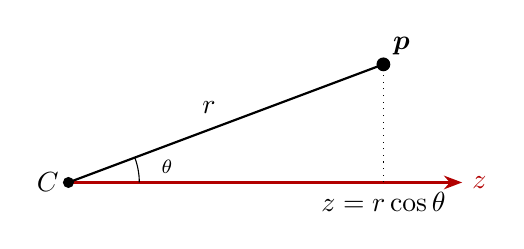
\begin{tikzpicture}[>=Stealth]
\draw[->,thick,red!70!black] (0,0)--(5,0) node[right]{$z$};
\fill (0,0) circle(2pt) node[left]{$C$};
\fill (4,1.5) circle(2.5pt) node[above right]{$\bm p$};
\draw[thick] (0,0)--(4,1.5) node[midway,above left]{$r$};
\draw[dotted] (4,0)--(4,1.5);
\node[below] at (4,0) {$z=r\cos\theta$};
\draw (0.9,0) arc(0:20.6:0.9); \node at (1.25,0.2) {\scriptsize $\theta$};
\end{tikzpicture}
\caption{Left: LiDAR and camera frames related by $\mathbf T_{cl}$ (redrawn from slide 19). Right: range $r$ versus depth $z$ (original figure).}
\end{figure}
 

\begin{figure}[H]
	\centering
	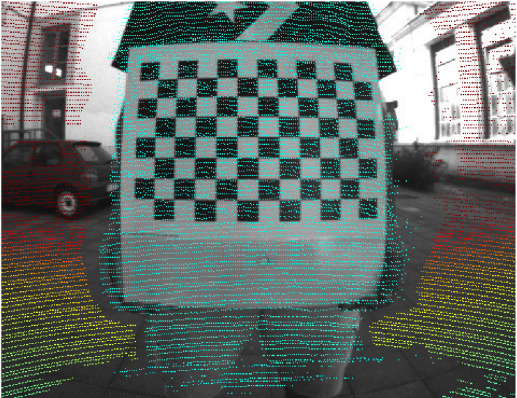
\includegraphics[width=1.0\linewidth]{1790768138707.png}
	\caption{grayscale image of a checkerboard target with LiDAR points projected onto it, colored by depth}\label{fig:1790768138707}
\end{figure}
 
\begin{algorithm}[LiDAR cloud to sparse depth map]
Input: points $\{\bm p^l_j\}$, intrinsics $\bm K$, extrinsics $(\bm R_{cl},\bm t_{cl})$, image size.
\begin{enumerate}[nosep]
\item Initialize $\bm D\leftarrow 0$ everywhere (``no measurement'').
\item For each point: $\bm p^c=\bm R_{cl}\bm p^l+\bm t_{cl}$; skip if $p^c_z\le0$ (behind the camera).
\item $\xt_s=\bm\pi(\bm K\bm p^c)$, round to a pixel; skip if outside the image.
\item If $\bm D[\bm x_s]=0$ or $p^c_z<\bm D[\bm x_s]$, set $\bm D[\bm x_s]\leftarrow p^c_z$.
\end{enumerate}
\end{algorithm}
 
\begin{intuition}
Step 4 is one common rule for ``points that fall in the same pixel'' (keep the nearest, as a z-buffer does); the slide only says such a rule is needed. Valid depths are strictly positive ($\bm D:\Omega\to\R_{>0}$), so $0$ can safely mark ``no return'' without colliding with a genuine measurement -- matching the earlier warning that a missing return is not a zero depth. Also remember that the result is \emph{sparse}: most pixels stay $0$.
\end{intuition}
 
% =====================================================================
\section{From Recovery to Prediction \slides{20--22}}
% =====================================================================
\emph{Paying with a prior.} One image does not determine depth. People judge it anyway, so they are supplying an assumption. This section turns that observation into a prior.
 
\subsection{Monocular Cues in Human Vision \slides{21}}
 
Not all 3D structures are equally likely, and human vision exploits that regularity through seven classic cues:
\begin{enumerate}[nosep]
\item linear perspective, \item relative size / position, \item texture gradient, \item occlusion (the occluded object is farther), \item aerial perspective, \item light and shadows, \item blur and defocus.
\end{enumerate}
 

\begin{figure}[H]
	\centering
	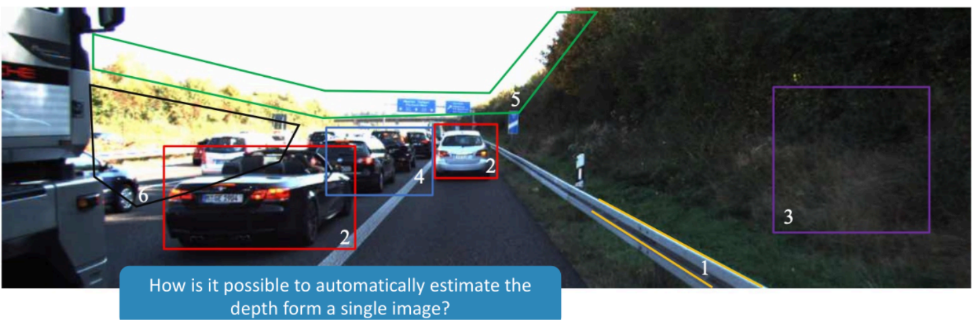
\includegraphics[width=1.0\linewidth]{1790768210811.png}
	\caption{driving image (highway scene) with the seven cues outlined and numbered}\label{fig:1790768210811}
\end{figure}
 
\begin{intuition}
None of these is a measurement. Each is an \emph{assumption about how scenes are usually arranged}: parallel lines meet, near things are big, far things are hazy. They work because the world is not a uniformly random set of 3D structures.
\end{intuition}
 
\subsection{Depth Prediction as a Prior \slides{22}}
 
\begin{proposition}[Bayesian view of single-image depth]\label{prop:bayes}
\[
p(\bm D\mid \bm I)\;\propto\; p(\bm I\mid \bm D)\,p(\bm D).
\]
The likelihood term is nearly flat along each ray (this is the ill-posedness of \S3.1), so the posterior is dominated by the prior $p(\bm D)$. Hence single-image depth is \emph{predicted} rather than \emph{recovered}, and a method is a claim about which scenes are likely.
\end{proposition}
 
\begin{intuition}
The likelihood asks: ``does this depth map explain the picture?'' Along a ray, every depth explains the pixel equally well, so the picture alone cannot vote. The only thing left to break ties is what depth maps \emph{usually look like} -- and people reading depth from a single photograph is everyday evidence that such a prior exists and is learnable. Where the learned one fails is the topic of \S3.8.
\end{intuition}
 
% =====================================================================
\section{Cues in Closed Form \slides{23--26}}
% =====================================================================
\emph{The prior, written in closed form.} Vanishing points, apparent size and vertical position each follow in one line from the projection equation.
 
\subsection{Vanishing Points \slides{24}}
 
Parallel 3D lines converge in the image; the horizon is the image of the line at infinity of the ground plane. A vanishing point is the image of a \emph{direction}, not of a location; every set of parallel lines has its own, and for a given plane they all lie on one line.
 
\begin{proposition}[Vanishing point of a direction]\label{prop:vp}
Let $\bm d\in\R^3$ be a 3D direction. Its image $\bm v$ satisfies
\[
\lambda\,\bm v=\bm K\,[\bm R\mid\bm t]\begin{pmatrix}\bm d\\0\end{pmatrix}=\bm K\bm R\,\bm d .
\]
\end{proposition}
\begin{proof}
A direction is a point at infinity, homogeneous coordinates $(\bm d,0)$. In the product $[\bm R\mid\bm t](\bm d,0)^\top=\bm R\bm d+\bm t\cdot0$ the translation is multiplied by zero and drops out. \qedhere
\end{proof}
 
\begin{corollary}
The horizon moves with camera \textbf{pitch and roll} only; translation does not move it.
\end{corollary}
 
\begin{example}[Horizon row for a pitched camera -- extra worked case]
Take zero roll, image $y$ pointing down, and pitch the camera up by $\theta$. The level forward direction has camera-frame coordinates $\bm R\bm d=(0,\sin\theta,\cos\theta)^\top$, so $\bm K\bm R\bm d$ gives the horizon row $y_h=c_y+f\tan\theta$: pitching up moves the horizon \emph{down} in the image.
\end{example}
 
\begin{figure}[htbp]
\centering
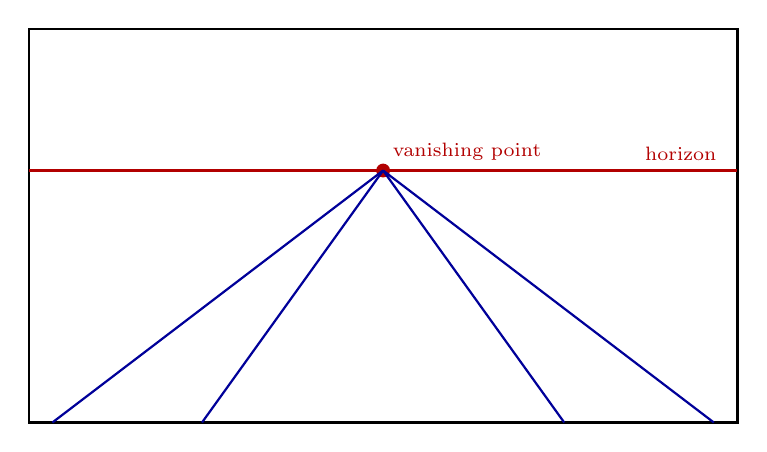
\begin{tikzpicture}[>=Stealth]
\draw[thick] (0,0) rectangle (9,5);
\draw[red!70!black,thick] (0,3.2)--(9,3.2) node[pos=0.92,above]{\scriptsize horizon};
\coordinate (V) at (4.5,3.2);
\fill[red!70!black] (V) circle(2.5pt) node[above right]{\scriptsize vanishing point};
\foreach \x in {0.3,2.2,6.8,8.7}{ \draw[blue!60!black,thick] (\x,0)--(V); }
\end{tikzpicture}
\caption{Original schematic (the slide shows a photograph, see below): parallel lines on the ground plane meet on the horizon.}
\end{figure}

 
\begin{figure}[H]
	\centering
	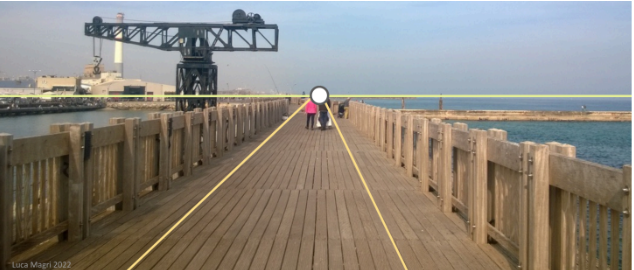
\includegraphics[width=1.0\linewidth]{1790768279993.png}
	\caption{photo of a wooden pier with yellow lines converging to a vanishing point on the horizon}\label{fig:1790768279993}
\end{figure}

\begin{intuition}
The translation drops out because a direction has no position: walking sideways does not change where the rails converge, only tilting the camera does. The slide adds a warning to remember: \emph{a network later on does not respect this} (\S3.8).
\end{intuition}
 
\subsection{Apparent Size \slides{25}}
 
\begin{proposition}[Depth from apparent size]\label{prop:size}
If the true height $H$ of an object is known and its image height is $h$ (in pixels), then
\[
z=\frac{f\,H}{h}.
\]
\end{proposition}
\begin{proof}
The camera center, the top and the bottom of the object form a triangle similar to the one formed by the center and the image of the object: $h/f=H/z$. \qedhere
\end{proof}
 
\begin{figure}[htbp]
\centering
\begin{tikzpicture}[>=Stealth]
\fill (0,0) circle(2pt) node[left]{$C$};
\draw[->,red!70!black,thick] (0,0)--(8.6,0) node[right]{$z$};
\draw[thick,black!60] (2,-0.5)--(2,1.2);
\draw[very thick,blue!60!black] (7,0)--(7,2);
\node[blue!60!black,right] at (7,1) {$H$};
\draw[dashed] (0,0)--(7,2);
\draw[very thick,blue!60!black] (2,0)--(2,0.571);
\node[blue!60!black,left] at (2,0.32) {$h$};
\draw[<->] (0,-0.7)--(2,-0.7) node[midway,below]{$f$};
\draw[<->] (0,-1.4)--(7,-1.4) node[midway,below]{$z$};
\end{tikzpicture}
\caption{Apparent size (redrawn from slide 25, side view).}
\end{figure}
 
\begin{example}
A car $H=1.5$\,m tall that appears $h=50$\,px tall with $f=700$\,px is at $z=700\cdot1.5/50=21$\,m.
\end{example}
 
\begin{intuition}
This works on driving data because almost everything in it is a car, a truck or a pedestrian, and those have known sizes: the \emph{prior about sizes} is doing the work. It fails for objects of unknown size -- the giant bench of \S3.1 again.
\end{intuition}
 
\subsection{Vertical Position \slides{26}}
 
\begin{proposition}[Depth from the ground contact point]\label{prop:vertical}
On a flat ground plane with known camera height $Y$, an object touching the ground at image row $y_s$ (horizon row $y_h$) has depth
\[
z=\frac{f\,Y}{y_s-y_h}.
\]
\end{proposition}
\begin{proof}
For a level camera, the ground point has camera-frame vertical coordinate $Y$ (below the camera) and depth $z$; projection gives $y_s-y_h=fY/z$. Solve for $z$. \qedhere
\end{proof}
 
\begin{figure}[htbp]
\centering
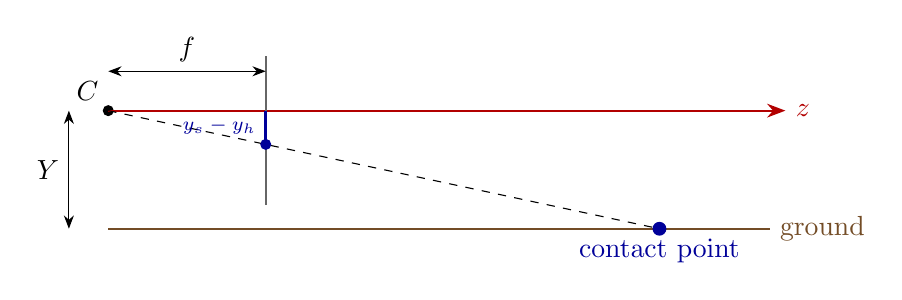
\begin{tikzpicture}[>=Stealth]
\fill (0,0) circle(2pt) node[above left]{$C$};
\draw[->,red!70!black,thick] (0,0)--(8.6,0) node[right]{$z$};
\draw[thick,black!60] (2,-1.2)--(2,0.7);
\draw[thick,brown!60!black] (0,-1.5)--(8.4,-1.5) node[right]{ground};
\draw[dashed] (0,0)--(7,-1.5);
\fill[blue!60!black] (7,-1.5) circle(2.5pt) node[below]{contact point};
\fill[blue!60!black] (2,-0.4286) circle(2pt);
\draw[very thick,blue!60!black] (2,0)--(2,-0.4286);
\node[left,blue!60!black] at (2,-0.2) {\scriptsize $y_s-y_h$};
\draw[<->] (-0.5,0)--(-0.5,-1.5) node[midway,left]{$Y$};
\draw[<->] (0,0.5)--(2,0.5) node[midway,above]{$f$};
\end{tikzpicture}
\caption{Vertical position (redrawn from slide 26, side view; horizon = optical axis for a level camera).}
\end{figure}
 
\begin{corollary}[Sensitivity]
Differentiating, $\delta z=z^2\,\delta y/(fY)$.
\end{corollary}
 
\begin{example}
$f=700$\,px, $Y=1.65$\,m, contact point $40$\,px below the horizon: $z=700\cdot1.65/40\approx28.9$\,m. A one-pixel error moves this by $z^2/(fY)\approx0.73$\,m.
\end{example}
 
\begin{intuition}
No knowledge of the object is required, only its contact point with the ground; but \emph{the assumptions carry the estimate}: flat ground, known camera height, known horizon. Note the resemblance to Proposition~\ref{prop:errlaw}: the error also grows as $z^2$, with the camera height $Y$ playing the role of a baseline (a remark of these notes, not on the slide). Cues near the horizon are extremely sensitive.
\end{intuition}
 
% =====================================================================
\section{Supervised Single-View Depth \slides{27--35}}
% =====================================================================
\emph{Paying with a prior, part two.} Fitting the prior requires an architecture, a loss that respects the scale ambiguity, and measured depth data.
 
\subsection{The Supervised Setup \slides{28}}
 
\begin{definition}[Supervised depth learning]
A training set of image / depth-map pairs, and a network from $3\times H\times W$ to $1\times H\times W$ trained with a per-pixel loss:
\[
\mathrm{TR}=\{(\bm I_i,\bm D_i)\}_{i=1}^{N},\qquad \hat{\bm D}=f_\theta(\bm I).
\]
\end{definition}
 
\begin{figure}[htbp]
\centering
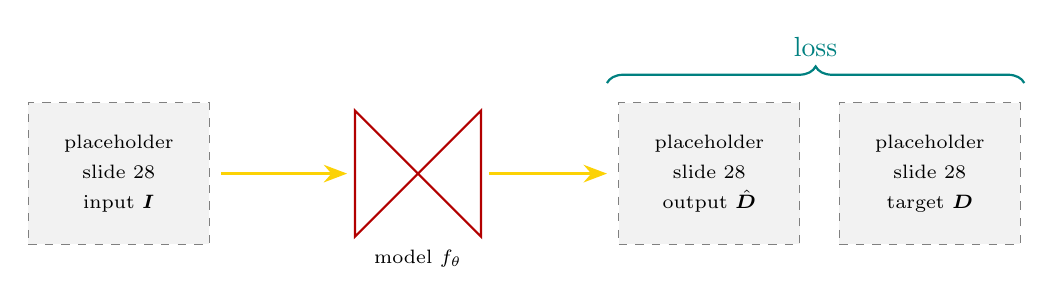
\begin{tikzpicture}[>=Stealth]
\node[draw=black!50,dashed,fill=black!5,minimum width=2.3cm,minimum height=1.8cm,align=center] (I) at (0,0) {\scriptsize placeholder\\[-1pt]\scriptsize slide 28\\[-1pt]\scriptsize input $\bm I$};
\draw[red!70!black,thick] (3,0.8)--(4.6,-0.8)--(4.6,0.8)--(3,-0.8)--cycle;
\node[below] at (3.8,-0.85) {\scriptsize model $f_\theta$};
\node[draw=black!50,dashed,fill=black!5,minimum width=2.3cm,minimum height=1.8cm,align=center] (P) at (7.5,0) {\scriptsize placeholder\\[-1pt]\scriptsize slide 28\\[-1pt]\scriptsize output $\hat{\bm D}$};
\node[draw=black!50,dashed,fill=black!5,minimum width=2.3cm,minimum height=1.8cm,align=center] (T) at (10.3,0) {\scriptsize placeholder\\[-1pt]\scriptsize slide 28\\[-1pt]\scriptsize target $\bm D$};
\draw[->,very thick,yellow!70!orange] (1.3,0)--(2.9,0);
\draw[->,very thick,yellow!70!orange] (4.7,0)--(6.2,0);
\draw[decorate,decoration={brace,amplitude=6pt},teal,thick] (6.2,1.15)--(11.5,1.15) node[midway,above=6pt,teal]{loss};
\end{tikzpicture}
\caption{The supervised setup (redrawn from slide 28; the two depth maps are photographs to copy from the slide).}
\end{figure}
 
\begin{intuition}
Data, network and per-pixel loss are the whole recipe; the slide's summary is that \emph{every remaining design decision is inside the loss} (\emph{what} counts as a correct prediction when scale is unobservable).
\end{intuition}
 
\subsection{Three Datasets \slides{29}}
 
Each of the three sits in a different cell of the principles table: a projected-pattern camera, a scanning laser, and triangulation with no known baseline.
 
\begin{itemize}
\item \textbf{NYU Depth v2}: indoor, from a structured-light depth camera, with its raw depth \emph{inpainted} to give a dense label.
\item \textbf{KITTI}: driving, LiDAR projected into the camera as in \S3.4.
\item \textbf{MegaDepth}: internet photo collections through structure from motion and multi-view stereo. Dense, varied, and \emph{scale-ambiguous by construction}.
\end{itemize}
 
These are the $\bm D_i$ of the previous slide. Each inherits the error sources of the sensor that produced it, and the last carries no metric scale at all -- which is what the next two methods are designed around.
 
\begin{table}[htbp]
\centering\footnotesize
\begin{tabular}{lllllr}
\toprule
Dataset & Annotation & Depth type & Accuracy & Diversity & \# images\\
\midrule
DIML Indoor & RGB-D & metric & medium & medium & 220K\\
MegaDepth & SfM & no scale & medium & medium & 130K\\
ReDWeb & stereo & no scale \& shift & medium & high & 3600\\
WSVD & stereo & no scale \& shift & medium & high & 1.5M\\
3D Movies & stereo & no scale \& shift & medium & high & 75K\\
DIW & user clicks & ordinal pair & low & high & 496K\\
ETH3D & laser & metric & high & low & 454\\
Sintel & synthetic & (metric) & high & medium & 1064\\
KITTI & laser/stereo & metric & medium & low & 93K\\
NYUDv2 & RGB-D & metric & medium & low & 407K\\
TUM-RGBD & RGB-D & metric & medium & low & 80K\\
\bottomrule
\end{tabular}
\caption{Trimmed transcription of the dataset table on slide 29 (the indoor/outdoor/dynamic/video/dense check-mark columns are omitted; copy the full table from the slide if needed).}
\end{table}
 
\begin{intuition}
Every dataset is a \emph{sensor's opinion} of depth. NYU inherits the holes and inpainting of a structured-light camera, KITTI inherits LiDAR sparsity and flying points, MegaDepth inherits SfM's arbitrary scale. Datasets with ``no scale \& shift'' or ``ordinal'' labels cannot be trained on with a plain L2 loss: the loss has to be told which ambiguity to ignore.
\end{intuition}
 
\subsection{The Scale-Invariant Loss \slides{30}}
 
The direct choice, $\mathcal D(\bm D,\hat{\bm D})=\|\bm D-\hat{\bm D}\|_2^2$, penalizes the network for a global scale the image does not determine. What is required is a loss invariant to that scale:
\[
\mathcal D(\bm y,\bm y^\ast)=\mathcal D(s\bm y,\bm y^\ast)\quad\forall s>0 .
\]
 
\begin{definition}[Eigen--Puhrsch--Fergus scale-invariant loss (NIPS 2014)]
Mean squared error in log space, plus a per-image offset:
\[
\mathcal D(\bm y,\bm y^\ast)=\frac1n\sum_{i=1}^n\big(\log y_i-\log y^\ast_i+\alpha\big)^2,
\qquad
\alpha=\frac1n\sum_{i=1}^n\big(\log y^\ast_i-\log y_i\big).
\]
\end{definition}
 
\begin{lemma}[Closed form and invariance]\label{lem:si}
Write $d_i=\log y_i-\log y^\ast_i$. Then $\alpha=-\bar d$ minimizes the expression over all offsets, and
\[
\mathcal D(\bm y,\bm y^\ast)=\frac1n\sum_i d_i^2-\frac1{n^2}\Big(\sum_i d_i\Big)^2=\operatorname{Var}(d_i).
\]
Moreover $\mathcal D(s\bm y,\bm y^\ast)=\mathcal D(\bm y,\bm y^\ast)$ for every $s>0$.
\end{lemma}
\begin{proof}
Differentiating $\sum_i(d_i+\alpha)^2$ in $\alpha$ and setting to zero gives $\alpha=-\bar d$; substituting yields $\frac1n\sum(d_i-\bar d)^2$, which is the stated variance. Replacing $\bm y$ by $s\bm y$ adds the constant $\log s$ to every $d_i$; a variance does not change under a constant shift. \qedhere
\end{proof}
 
\begin{figure}[htbp]
\centering
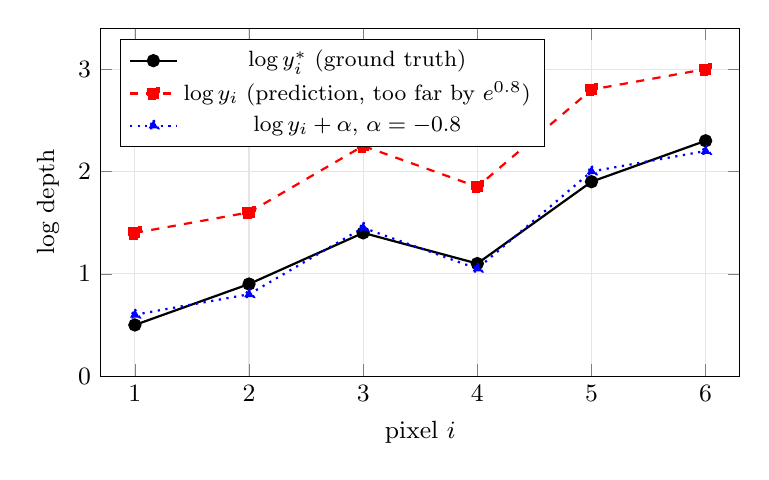
\begin{tikzpicture}
\begin{axis}[width=0.8\linewidth,height=6cm,xlabel={pixel $i$},ylabel={log depth},xmin=0.7,xmax=6.3,ymin=0,ymax=3.4,
  legend style={at={(0.03,0.97)},anchor=north west,font=\footnotesize},grid=both,grid style={gray!20}]
\addplot[black,thick,mark=*] coordinates {(1,0.5)(2,0.9)(3,1.4)(4,1.1)(5,1.9)(6,2.3)};
\addlegendentry{$\log y^\ast_i$ (ground truth)}
\addplot[red,thick,dashed,mark=square*] coordinates {(1,1.4)(2,1.6)(3,2.25)(4,1.85)(5,2.8)(6,3.0)};
\addlegendentry{$\log y_i$ (prediction, too far by $e^{0.8}$)}
\addplot[blue,thick,dotted,mark=triangle*] coordinates {(1,0.6)(2,0.8)(3,1.45)(4,1.05)(5,2.0)(6,2.2)};
\addlegendentry{$\log y_i+\alpha$, $\alpha=-0.8$}
\end{axis}
\end{tikzpicture}
\caption{Original toy example (not on the slides). The prediction has the right shape but a wrong global scale. Naive log-MSE would be $\approx0.646$; the scale-invariant loss, after aligning by $e^{\alpha}$, is only $\approx0.0058$.}
\end{figure}
 
\begin{intuition}
In log space a wrong \emph{scale} becomes a constant \emph{offset}, and the loss subtracts the best constant offset before looking at the errors. So only the \emph{shape} of the depth map is judged. Two side remarks from the slide: log space stops far pixels (numerically large) from dominating, and $e^{\alpha}\bm y$ is the scalar multiple that best aligns the prediction to the ground truth -- every scalar multiple of $\bm y$ scores identically.
\end{intuition}
 
\subsection{Output Spaces \slides{31}}
 
Five quantities a depth network can predict differ in how many unknowns are left free, and in \emph{what the free parameters act on}.
 
\begin{table}[htbp]
\centering\small
\begin{tabularx}{\linewidth}{@{}p{0.3cm}Ycp{3.1cm}Y@{}}
\toprule
& output & free param. & aligned by & trained this way to\\
\midrule
1 & metric depth & 0 & nothing & plan and measure\\
2 & scale-invariant depth & 1 ($s$) & one scale & share one scale per scene\\
3 & affine-invariant disparity & 2 ($s,t$) & scale and shift & mix datasets with no common zero\\
4 & affine-invariant depth & 2 ($s,t$) & scale and shift & mix datasets in depth (3.11)\\
5 & ordinal & any monotone map & nothing & rank only\\
\bottomrule
\end{tabularx}
\caption{Output spaces (slide 31). Scale-invariant: $\hat y\approx s\,y^\ast$; affine-invariant: $\hat q\approx s\,q^\ast+t$ with $q=1/y$ for disparity.}
\end{table}
 
These are routinely conflated: Eigen's log-space is \emph{one} parameter, affine invariance \emph{two}. The affine row appears twice because the same pair $(s,t)$ can act on disparity or on depth, and the two differ in 3D (next subsection). Benchmarks align the free parameters against the ground truth first, then score with $\delta$ and AbsRel, so a model is scored on \emph{shape, not on meters}.
 
\begin{example}[Standard metrics, background]
$\mathrm{AbsRel}=\frac1n\sum_i|\hat y_i-y^\ast_i|/y^\ast_i$, and $\delta_1$ is the fraction of pixels with $\max(\hat y_i/y^\ast_i,\,y^\ast_i/\hat y_i)<1.25$; both are computed after the alignment above.
\end{example}
 
\subsection{Affine Invariance in Disparity and in Depth \slides{32}}
 
\begin{proposition}[Affine map in disparity = projective map in space]\label{prop:affdisp}
An affine map in inverse depth,
\[
\frac1z\;\longmapsto\;\frac{s}{z}+t\quad\Longleftrightarrow\quad z\;\longmapsto\;\frac{z}{s+t\,z},
\]
is a nonlinear map in depth. Back-projecting the transformed depth gives $\hat{\bm p}=\bm p/(s+t\,p_z)$, which is a \emph{projective} map of space: planes remain planes.
\end{proposition}
\begin{proof}
$s/z+t=(s+tz)/z$, so $z\mapsto z/(s+tz)$. Back-projection by \eqref{eq:backproj}: $\hat{\bm p}=\frac{z}{s+tz}\Kinv\xt_s=\bm p/(s+tp_z)$. To see planes stay planes, let $\bm a^\top\bm p=c$ and $w=s+tp_z$. From $\hat{\bm p}=\bm p/w$ we get $\hat p_z=p_z/w$, hence $p_z=s\hat p_z/(1-t\hat p_z)$ and $w=s/(1-t\hat p_z)$, so $\bm p=w\hat{\bm p}$. Substituting, $s\,\bm a^\top\hat{\bm p}=c\,(1-t\hat p_z)$, which is linear in $\hat{\bm p}$. \qedhere
\end{proof}
 
\begin{figure}[htbp]
\centering
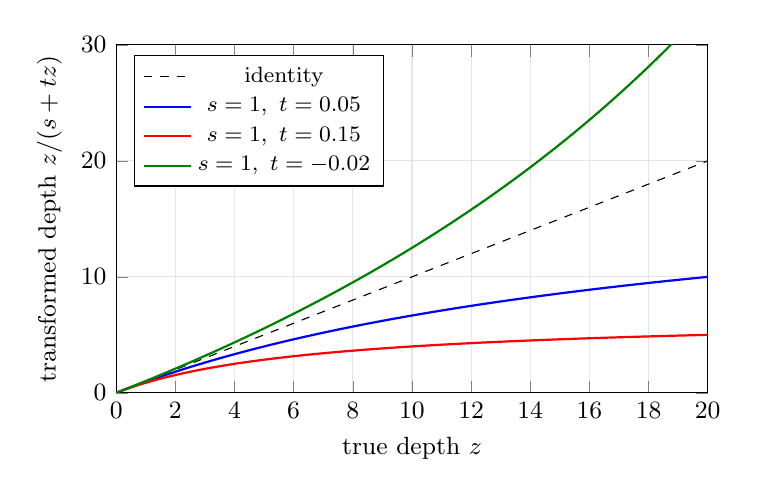
\begin{tikzpicture}
\begin{axis}[width=0.75\linewidth,height=6cm,xlabel={true depth $z$},ylabel={transformed depth $z/(s+tz)$},xmin=0,xmax=20,ymin=0,ymax=30,
  legend style={at={(0.03,0.97)},anchor=north west,font=\footnotesize},grid=both,grid style={gray!20}]
\addplot[black,dashed,domain=0:20,samples=2]{x};
\addlegendentry{identity}
\addplot[blue,thick,domain=0:20,samples=60]{x/(1+0.05*x)};
\addlegendentry{$s=1,\ t=0.05$}
\addplot[red,thick,domain=0:20,samples=60]{x/(1+0.15*x)};
\addlegendentry{$s=1,\ t=0.15$}
\addplot[green!50!black,thick,domain=0:20,samples=60]{x/(1-0.02*x)};
\addlegendentry{$s=1,\ t=-0.02$}
\end{axis}
\end{tikzpicture}
\caption{Original figure (not on the slides): an affine map in disparity acts on \emph{depth} as $z\mapsto z/(s+tz)$, a compressive or expansive warp, not a rescaling.}
\end{figure}
 
\begin{intuition}
A ground plane is therefore \emph{tilted, not bent}: you can decide a scale and shift wrongly, and flat things stay flat but the world may look sheared toward or away from the camera. An affine map in depth itself would instead be $z\mapsto sz+t$, a rigid stretch and translation along the ray. The two choices give the same 2-parameter count but \emph{different 3D geometry} -- the reason the table lists the affine row twice.
\end{intuition}
 
\subsection{MiDaS: Mixing the Datasets \slides{33}}
 
No single dataset covers the visual world, so MiDaS trains on several. The obstacle is that they disagree about what they measure (metric, no scale, no scale and shift, ordinal, ...). Its recipe:
\begin{itemize}
\item predict in \textbf{disparity space} (inverse depth up to scale and shift);
\item train with a \textbf{scale-and-shift-invariant loss}, where the alignment $(s,t)$ is a least-squares fit solved \emph{in closed form per image};
\item add a \textbf{multi-scale gradient matching} term, which is the gradient loss again, at four resolutions.
\end{itemize}
The output space is the affine-invariant \emph{disparity} row of the table, not the affine-invariant \emph{depth} row under it.
 
\begin{lemma}[Closed-form alignment]\label{lem:ssi}
For predictions $\hat q_i$ and targets $q^\ast_i$, the pair
\[
(s,t)=\arg\min_{s,t}\sum_i\big(s\,\hat q_i+t-q^\ast_i\big)^2
\]
is $s=\dfrac{\operatorname{Cov}(\hat q,q^\ast)}{\operatorname{Var}(\hat q)}$, $\;t=\bar q^\ast-s\,\bar{\hat q}$ (assuming $\operatorname{Var}(\hat q)>0$).
\end{lemma}
\begin{proof}
Setting $\partial/\partial t=0$ gives $t=\bar q^\ast-s\bar{\hat q}$. Setting $\partial/\partial s=0$: $s\sum\hat q_i^2+t\sum\hat q_i=\sum\hat q_iq_i^\ast$. Substituting $t$ and dividing by $n$: $s(\overline{\hat q^2}-\bar{\hat q}^2)=\overline{\hat qq^\ast}-\bar{\hat q}\bar q^\ast$. \qedhere
\end{proof}
 
The loss is then evaluated on the residual \emph{after} alignment. The gradient matching term, in its standard form, penalizes gradients of the aligned residual $R^k$ at each of the $K=4$ scales $k$: $\frac1M\sum_{k=1}^{K}\sum_i(|\nabla_xR^k_i|+|\nabla_yR^k_i|)$ (form from the original MiDaS paper; the slide only says ``the gradient loss again, at four resolutions'').
 
\begin{figure}[htbp]
\centering
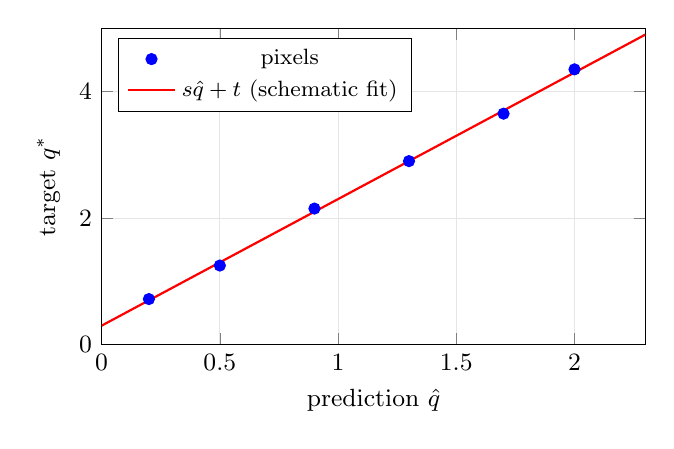
\begin{tikzpicture}
\begin{axis}[width=0.7\linewidth,height=5.6cm,xlabel={prediction $\hat q$},ylabel={target $q^\ast$},xmin=0,xmax=2.3,ymin=0,ymax=5,grid=both,grid style={gray!20},
  legend style={at={(0.03,0.97)},anchor=north west,font=\footnotesize}]
\addplot[only marks,mark=*,blue] coordinates {(0.2,0.72)(0.5,1.25)(0.9,2.15)(1.3,2.9)(1.7,3.65)(2.0,4.35)};
\addlegendentry{pixels}
\addplot[red,thick,domain=0:2.3,samples=2]{2*x+0.3};
\addlegendentry{$s\hat q+t$ (schematic fit)}
\end{axis}
\end{tikzpicture}
\caption{Original schematic (not on the slides): per-image least-squares alignment of a prediction to targets that use a different scale and zero.}
\end{figure}
 
\begin{intuition}
Each training image gets its \emph{own} best-fit $(s,t)$ before the network is judged, like a teacher who marks a student's drawing after allowing it to be enlarged and moved on the page. That is what lets one network learn from a metric laser dataset, an up-to-scale SfM dataset and a stereo-movie dataset at the same time. Working in \emph{disparity} matters because an unknown rig only contributes an unknown scale there (Corollary~\ref{cor:unknownb}).
\end{intuition}
 
\subsection{Depth Anything V2 \slides{34}}
 
Labeled depth data is the bottleneck, so the second version removes the requirement for it (the first version also trained on labeled real data).
 
\begin{algorithm}[Teacher--student training]
\begin{enumerate}[nosep]
\item Train a \textbf{teacher} on precise \emph{synthetic} images only, where depth is exact and complete.
\item Use the teacher to \textbf{pseudo-label} a very large set of unlabeled real photographs.
\item Train the \textbf{student} on those pseudo-labels.
\end{enumerate}
\end{algorithm}
 
Architecture and losses: encoder from self-supervised pretraining, decoder from dense prediction, and the \emph{same} scale-and-shift-invariant plus gradient-matching losses as MiDaS. The output space is affine-invariant inverse depth; metric models are a separate fine-tuning step on top.
 
\begin{figure}[htbp]
\centering
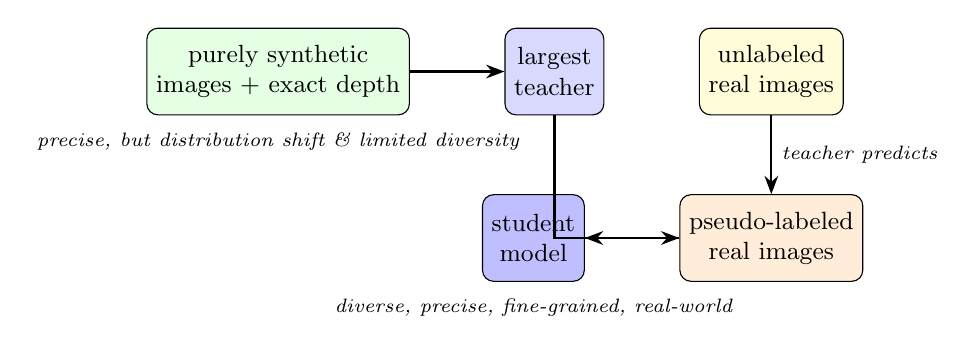
\begin{tikzpicture}[>=Stealth,node distance=6mm,
  box/.style={draw,rounded corners,minimum height=1.1cm,align=center,font=\small},
  tag/.style={font=\scriptsize\itshape}]
\node[box,fill=green!10] (syn) {purely synthetic\\images + exact depth};
\node[box,fill=blue!15,right=12mm of syn] (teach) {largest\\teacher};
\node[box,fill=yellow!15,right=12mm of teach] (unl) {unlabeled\\real images};
\node[box,fill=orange!15,below=10mm of unl] (pl) {pseudo-labeled\\real images};
\node[box,fill=blue!25,left=12mm of pl] (stud) {student\\model};
\draw[->,thick] (syn)--(teach);
\draw[->,thick] (unl)--(pl) node[midway,right,tag]{teacher predicts};
\draw[->,thick] (teach.south) |- (pl.west) ;
\draw[->,thick] (pl)--(stud);
\node[tag,below=1mm of syn]{precise, but distribution shift \& limited diversity};
\node[tag,below=1mm of stud]{diverse, precise, fine-grained, real-world};
\end{tikzpicture}
\caption{Depth Anything V2 pipeline (redrawn from slide 34).}
\end{figure}
 
\begin{intuition}
Synthetic images give \emph{perfect} labels but look unlike the real world; real photos look right but have no labels. The teacher transfers its precision to real photos through pseudo-labels, so the student sees real-world diversity with clean, fine-grained targets. The price: the student inherits what the teacher believes -- its prior -- rather than anything measured.
\end{intuition}
 
\subsection{Failure on Anamorphic Art \slides{35}}
 
Anamorphic street art is a flat pavement painted to look like a hole. The predicted depth map is wrong throughout, with no indication of uncertainty. Nothing has malfunctioned: the prior behaves as trained, on an input constructed to exploit it. \emph{The prior is both the method and the failure mode.}

 \begin{figure}[H]
	\centering
	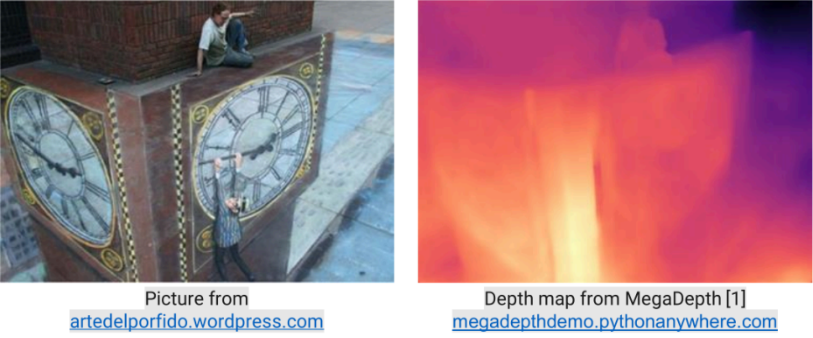
\includegraphics[width=1.0\linewidth]{1790768347386.png}
	\caption{left: photo of a street painting of a clock tower on pavement; right: predicted depth map from MegaDepth demo}\label{fig:1790768347386}
 \end{figure}

\begin{figure}[htbp]
\centering
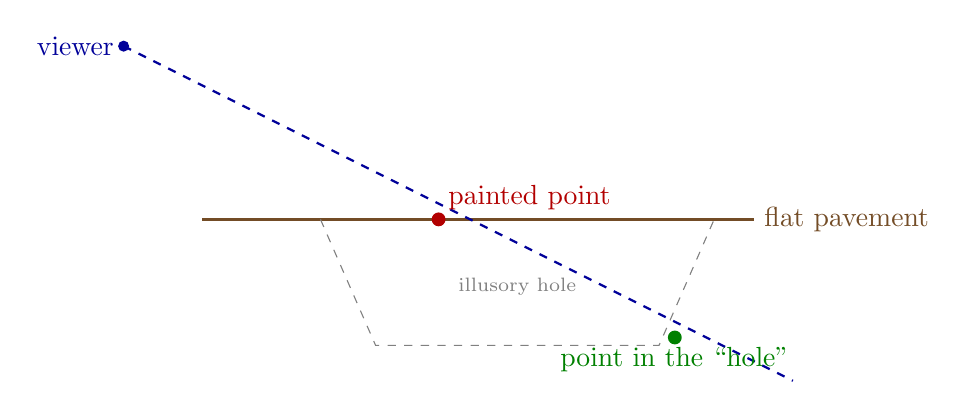
\begin{tikzpicture}[>=Stealth]
\fill[blue!60!black] (0,2.2) circle(2pt) node[left]{viewer};
\draw[very thick,brown!60!black] (1,0)--(8,0) node[right]{flat pavement};
\draw[dashed,thick,blue!60!black] (0,2.2)--(8.5,-2.05);
\fill[red!70!black] (4,0) circle(2.5pt) node[above right]{painted point};
\fill[green!50!black] (7,-1.5) circle(2.5pt) node[below]{point in the ``hole''};
\draw[dashed,gray] (2.5,0)--(3.2,-1.6)--(6.8,-1.6)--(7.5,0);
\node[gray] at (5,-0.85) {\scriptsize illusory hole};
\end{tikzpicture}
\caption{Original figure (not on the slides): from the painting's viewpoint the painted point on the flat ground and the point at the bottom of the imagined hole lie on the same ray (Proposition~\ref{prop:ray}). One image cannot distinguish them, so the network chooses the ``likely'' one.}
\end{figure}
 
\begin{intuition}
The picture is a concrete instance of the back-projected ray: the artist chooses a flat surface whose appearance is \emph{exactly} what a deep hole would look like from one viewpoint. Depth-from-one-image cannot know; it picks the answer its training data make most probable. Note also the ``no indication of uncertainty'': the network is confidently wrong.
\end{intuition}
 
% =====================================================================
\section{Cues Used by the Network \slides{36--39}}
% =====================================================================
\emph{What the prior turns out to be.} A monocular depth network is a prior fitted to a dataset. Three probes examine which image evidence that prior relies on.
 
\subsection{The Pasted-Car Experiment \slides{37}}
 
A car is cropped from the image and pasted back at a chosen ground contact point and a chosen scale, placing the two cues of \S3.6 in conflict: both correct (position \& size), \emph{position only}, or \emph{size only}. The finding (paraphrased): across four networks, the vertical position in the image wins over the apparent size of known obstacles.
\begin{itemize}
\item Position only tracks the true distance; size only does not.
\item The result holds across four networks.
\item Vertical position needs no object model and generalizes to objects absent from the training set.
\end{itemize}
 
 
\begin{figure}[H]
	\centering
	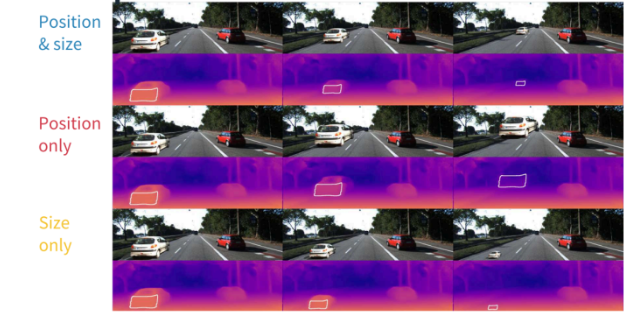
\includegraphics[width=1.0\linewidth]{1790768421548.png}
	\caption{grid of pasted-car examples (position \& size / position only / size only) with predicted depth maps}\label{fig:1790768421548}
\end{figure}

\begin{figure}[htbp]
\centering
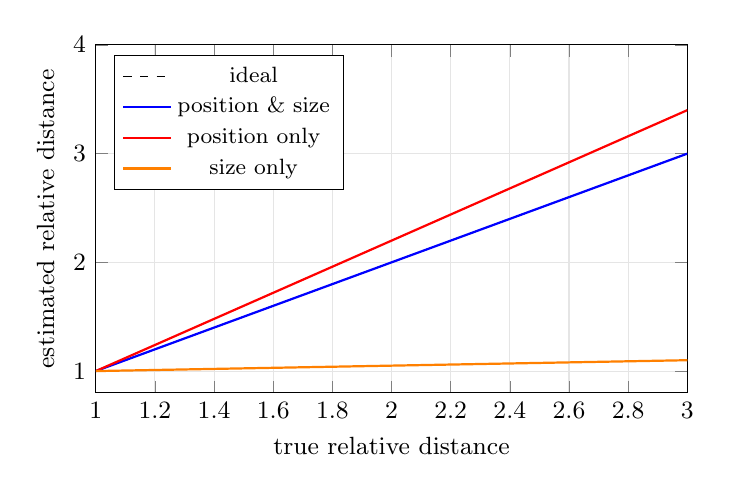
\begin{tikzpicture}
\begin{axis}[width=0.75\linewidth,height=6cm,xlabel={true relative distance},ylabel={estimated relative distance},xmin=1,xmax=3,ymin=0.8,ymax=4,
  legend style={at={(0.03,0.97)},anchor=north west,font=\footnotesize},grid=both,grid style={gray!20}]
\addplot[black,dashed,domain=1:3,samples=2]{x};
\addlegendentry{ideal}
\addplot[blue,thick,domain=1:3,samples=2]{1+1.0*(x-1)};
\addlegendentry{position \& size}
\addplot[red,thick,domain=1:3,samples=2]{1+1.2*(x-1)};
\addlegendentry{position only}
\addplot[orange,thick,domain=1:3,samples=2]{1+0.05*(x-1)};
\addlegendentry{size only}
\end{axis}
\end{tikzpicture}
\caption{\textbf{Qualitative schematic} after the plot on slide 37, not measured data: positional cues track the ideal line (with some overestimate and larger spread), size-only stays almost flat.}
\end{figure}
 
\begin{intuition}
The networks behave like the vertical-position cue of Proposition~\ref{prop:vertical}, not like Proposition~\ref{prop:size}. Sensible: vertical position works for \emph{anything} touching the ground, whereas size needs a size prior per object class. But it also means a car pasted ``floating'' higher in the frame is judged farther, even if it appears huge.
\end{intuition}
 
\subsection{Pitch and Roll \slides{38}}
 
A pitch change is simulated with a vertical crop and a roll with a rotated crop; both are recovered from the predicted depth. Findings: the networks \textbf{only partially} track camera orientation, and small pitch changes measurably disturb the estimated distance to obstacles.
 
\begin{figure}[htbp]
\centering
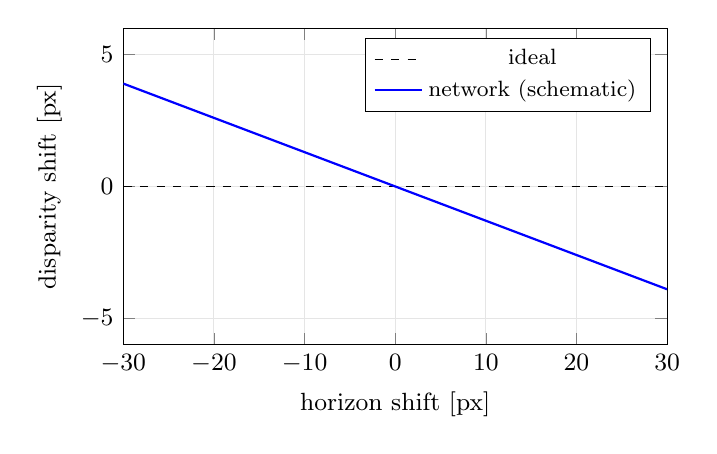
\begin{tikzpicture}
\begin{axis}[width=0.7\linewidth,height=5.6cm,xlabel={horizon shift [px]},ylabel={disparity shift [px]},xmin=-30,xmax=30,ymin=-6,ymax=6,grid=both,grid style={gray!20},
  legend style={at={(0.97,0.97)},anchor=north east,font=\footnotesize}]
\addplot[black,dashed,domain=-30:30,samples=2]{0};
\addlegendentry{ideal}
\addplot[blue,thick,domain=-30:30,samples=2]{-0.13*x};
\addlegendentry{network (schematic)}
\end{axis}
\end{tikzpicture}
\caption{\textbf{Qualitative schematic} after the plot on slide 38, not measured data: an ideal system would ignore the crop (zero shift), the networks' output drifts roughly linearly and opposite to the horizon shift.}
\end{figure}
 
\begin{intuition}
A crop does \emph{not} change an object's distance to the horizon, $y_s-y_h$, so by Proposition~\ref{prop:vertical} the true depth cannot change. But it does change the object's \emph{absolute} vertical position, and the predictions change with it. The network reads vertical image position, rather than distance to the horizon -- exactly the shortcut warned about in \S3.6, where the horizon depends on pitch and roll only.
\end{intuition}
 
\subsection{Dependence on the Training Camera \slides{39}}
 
A third probe: what happens when only the \emph{camera} changes. A network trained at one focal length predicts the wrong depth at another, with the scene held identical. The apparent-size relation (Proposition~\ref{prop:size}) contains $f$, and the network has absorbed the training value as a constant. Supplying the intrinsics to the network as extra input channels removes most of the error. The slide's summary: the prior is fitted to the training \emph{camera} as much as to the training \emph{scenes}.
 
\begin{proposition}[Idealized focal-length bias -- worked consequence, not on the slide]\label{prop:focal}
Suppose a network has absorbed $z=f_0H/h$ with the training focal length $f_0$. At test focal length $f$ the image height is $h'=fH/z$, so the predicted depth is
\[
\hat z=\frac{f_0H}{h'}=\frac{f_0}{f}\,z .
\]
\end{proposition}
 
\begin{figure}[htbp]
\centering
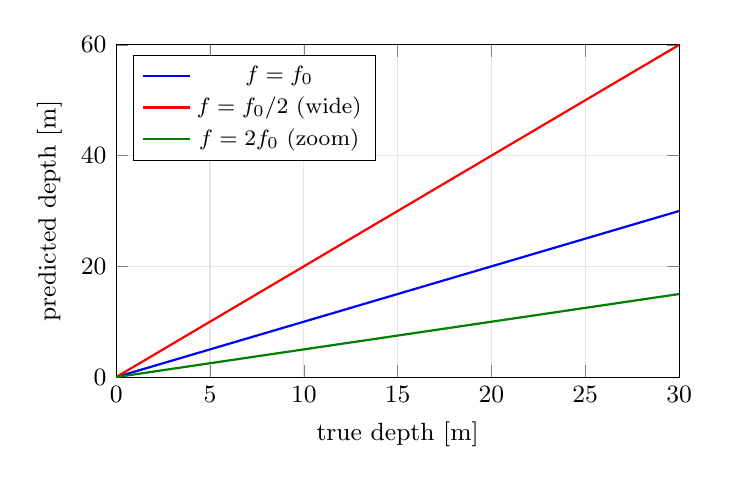
\begin{tikzpicture}
\begin{axis}[width=0.72\linewidth,height=5.8cm,xlabel={true depth [m]},ylabel={predicted depth [m]},xmin=0,xmax=30,ymin=0,ymax=60,grid=both,grid style={gray!20},
  legend style={at={(0.03,0.97)},anchor=north west,font=\footnotesize}]
\addplot[blue,thick,domain=0:30,samples=2]{x};
\addlegendentry{$f=f_0$}
\addplot[red,thick,domain=0:30,samples=2]{2*x};
\addlegendentry{$f=f_0/2$ (wide)}
\addplot[green!50!black,thick,domain=0:30,samples=2]{0.5*x};
\addlegendentry{$f=2f_0$ (zoom)}
\end{axis}
\end{tikzpicture}
\caption{Original figure (not on the slides): predicted depth under the idealization of Proposition~\ref{prop:focal}.}
\end{figure}
 
\begin{intuition}
Zooming in makes everything look bigger, and a network that silently assumes the training focal length reads ``bigger'' as ``closer''. This is a scale error, so it is precisely the kind of ambiguity metric prediction must resolve -- giving the network the intrinsics removes the hidden constant.
\end{intuition}

% =====================================================================
\section*{Next: Self-Supervision and a Generative Prior \slides{40}}
\addcontentsline{toc}{section}{Next: Self-Supervision and a Generative Prior \emph{(slide 40)}}

Part~I closes owing two debts: the prior was fitted to labels that a sensor had to measure, and mixing those labels cost two free parameters. Part~II removes the labels, then pays back the two numbers.

\section*{Part I in One Slide \slides{1--2}}
\addcontentsline{toc}{section}{Overview: Part I in One Slide \emph{(slides 1--2)}}
%=====================================================================
Part~I obtained depth in two ways and closed \emph{owing two debts}:
\begin{itemize}[nosep]
  \item \textbf{Time.} A laser measures range directly: metric and exact where it lands, but sparse, and it produces the labels everything else trains on.
  \item \textbf{A prior.} A network fitted to those labels is dense and cheap, but it \emph{predicts} rather than recovers depth. The prior was fitted to labels that a sensor had to measure.
\end{itemize}
Mixing labels of different origin moved the output down a table, at a cost of free parameters.

\begin{definition}[Output types and their free parameters]
A depth-like output is defined only up to a transformation, and each transformation leaves free parameters that something else must later fix.
\begin{center}\small
\begin{tabular}{@{}lcl@{}}\toprule
output & free parameters & aligned by\\\midrule
metric depth & 0 & nothing\\
scale-invariant depth & 1 & one scale $s$\\
affine-invariant disparity or depth & 2 & scale and shift $(s,t)$\\
ordinal & any monotone map & nothing\\\bottomrule
\end{tabular}
\end{center}
\end{definition}

\begin{intuition}
Each free parameter is a \emph{number a sensor must still supply}. If a network says ``this pixel is twice as far as that one'', it has told you shape but not meters. Example: the truth is $D=2.0\,\hat D+0.3$~m. A metric network outputs $D$ itself; an affine-invariant one outputs $\hat D$ and you need the pair $(2.0,\,0.3)$ to recover meters. The whole lecture is about who supplies those numbers: the baseline of a stereo rig, a large generative prior, or a handful of LiDAR returns.
\end{intuition}

%=====================================================================
\section{Supervision without Ground Truth \slides{3--6}}
%=====================================================================
This is section 3.9 of the lecture. Its thesis: \emph{a stereo pair supplies its own supervision, provided the warp connecting the two images is differentiable.}

\subsection{View Synthesis and the Backward Warp \slides{4}}
Training uses stereo pairs $\{(\bm I_L,\bm I_R)\}$ only; there is no depth anywhere in the training set. The objective is to reproduce one image of the pair from the other. Depth is the only internal quantity that makes this task solvable, so if the network solves it, depth is what it must have learned. This holds only where a pixel is \textbf{textured} and visible in \textbf{both} views; elsewhere the objective says nothing and a hand-written prior fills the gap.

\begin{definition}[Backward warp]
Given a disparity map $d(u,v)$ defined on the \emph{target} image, the backward warp synthesizes the target from the source by
\begin{equation}
\tilde{\bm I}_L(u,v)=\bm I_R\bigl(u-d(u,v),\,v\bigr).
\end{equation}
Every \emph{target} pixel is mapped to exactly one \emph{source} location.
\end{definition}

\begin{proposition}[Why the warp must be backward]
Forward mapping (pushing each source pixel to a target location) lets several sources land on one target pixel and leaves other target pixels empty: collisions and holes. Backward mapping assigns each target pixel exactly one value, which makes the warp a \emph{differentiable function} of $d$ rather than a scatter operation.
\end{proposition}

\begin{figure}[H]
\centering
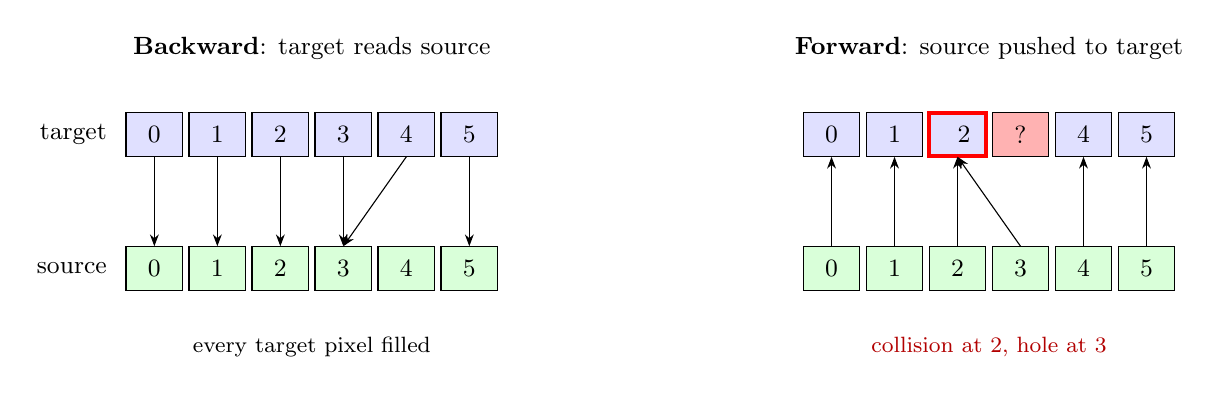
\begin{tikzpicture}[x=0.8cm,y=1cm,font=\small,
  pix/.style={draw,minimum width=0.72cm,minimum height=0.55cm,inner sep=0,fill=blue!12}]
\begin{scope}
 \node at (2.5,3.3) {\textbf{Backward}: target reads source};
 \foreach \i in {0,...,5}{\node[pix] (bt\i) at (\i,2.2){\i}; \node[pix,fill=green!15] (bs\i) at (\i,0.5){\i};}
 \node[anchor=east] at (-0.6,2.2){target}; \node[anchor=east] at (-0.6,0.5){source};
 \foreach \t/\s in {0/0,1/1,2/2,3/3,4/3,5/5}{\draw[-{Stealth[length=1.5mm]}] (bt\t.south)--(bs\s.north);}
 \node[font=\footnotesize,align=center] at (2.5,-0.5){every target pixel filled};
\end{scope}
\begin{scope}[xshift=8.6cm]
 \node at (2.5,3.3) {\textbf{Forward}: source pushed to target};
 \foreach \i in {0,...,5}{\node[pix] (ft\i) at (\i,2.2){\i}; \node[pix,fill=green!15] (fs\i) at (\i,0.5){\i};}
 \node[pix,fill=red!30] at (3,2.2){?};
 \node[pix,ultra thick,draw=red] at (2,2.2){\phantom{0}2};
 \foreach \s/\t in {0/0,1/1,2/2,3/2,4/4,5/5}{\draw[-{Stealth[length=1.5mm]}] (fs\s.north)--(ft\t.south);}
 \node[font=\footnotesize,align=center,text=red!70!black] at (2.5,-0.5){collision at 2, hole at 3};
\end{scope}
\end{tikzpicture}
\caption{Original 1D illustration of backward versus forward mapping (slide 4 shows the same effect on small coloured grids).}
\end{figure}

\begin{intuition}
Think of filling in a form versus mailing letters. Backward warping is the form: each target pixel asks \emph{``where in the other image should I look?''} and gets exactly one answer. Forward warping is the post office: every source pixel is mailed to an address; some mailboxes get two letters (collision), others none (hole), and ``two letters or none'' has no useful gradient. Note the sign convention: slide~4 writes $u-d$ for the left image as target, slide~5 writes $+d$ for a target/source pair set up the other way round; only the consistent use matters.
\end{intuition}

\subsection{Image Reconstruction as Supervision \slides{5}}
The pipeline of slide~5 has three steps: (1) a deep CNN predicts an inverse depth from the left image; (2) the right image is warped with it into a synthetic left image; (3) the reconstruction error against the real left image is the loss.

\begin{definition}[Disparity and photometric loss]
Under a rectified stereo rig with focal length $f$ and baseline $b$, the predicted inverse depth is the disparity
\begin{equation}
d(\bm p)=\frac{f\,b}{z(\bm p)}.
\end{equation}
The self-supervised loss compares the warped and real image,
\begin{equation}
\mathcal L_{\text{photo}}=\sum_{\bm p}\bigl\|\tilde{\bm I}(\bm p)-\bm I_L(\bm p)\bigr\|,\qquad \tilde{\bm I}(\bm p)=\bm I_R\bigl(\bm p+d(\bm p)\bigr).
\end{equation}
\end{definition}

\begin{figure}[H]
\centering
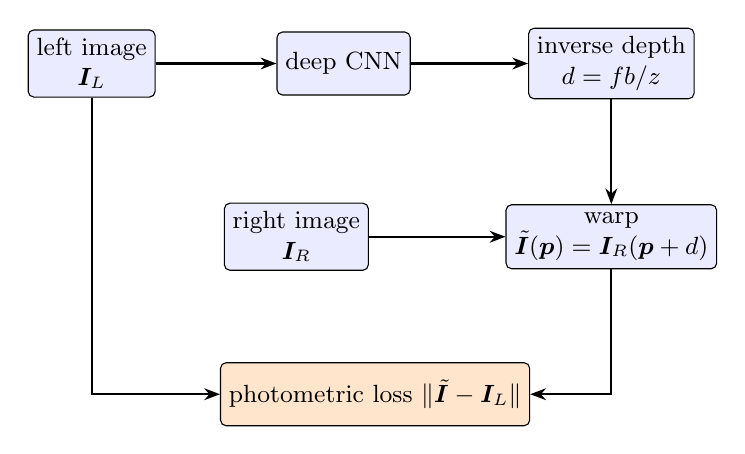
\begin{tikzpicture}[font=\small]
\node[box] (IL) at (0,0) {left image\\$\bm I_L$};
\node[box] (cnn) at (3.2,0) {deep CNN};
\node[box] (d) at (6.6,0) {inverse depth\\$d=fb/z$};
\node[box] (warp) at (6.6,-2.2) {warp\\$\tilde{\bm I}(\bm p)=\bm I_R(\bm p+d)$};
\node[box] (IR) at (2.6,-2.2) {right image\\$\bm I_R$};
\node[box,fill=orange!20] (loss) at (3.6,-4.2) {photometric loss $\|\tilde{\bm I}-\bm I_L\|$};
\draw[arr] (IL)--(cnn); \draw[arr] (cnn)--(d); \draw[arr] (d)--(warp);
\draw[arr] (IR)--(warp);
\draw[arr] (warp.south) |- (loss.east);
\draw[arr] (IL.south) |- (loss.west);
\end{tikzpicture}
\caption{Self-supervised stereo training (redrawn from slide 5). No depth label appears anywhere.}
\end{figure}

\begin{figure}[H]
	\centering
	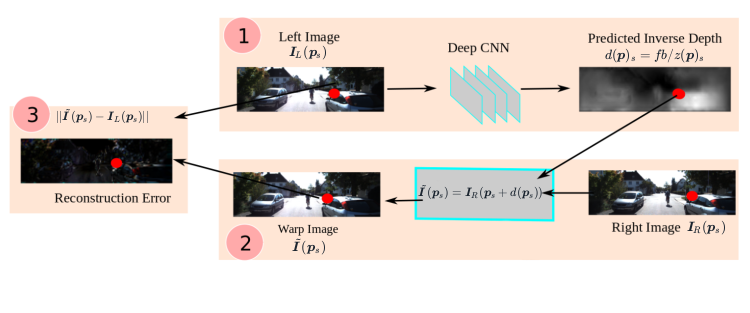
\includegraphics[width=1.0\linewidth]{1790765520552.png}
	\caption{the KITTI street scene: left image, predicted inverse-depth map, warped image and reconstruction-error map (steps 1--3, with the red marker point)}\label{fig:1790765520552}
\end{figure}
\begin{intuition}
Depth is the \emph{only} unknown the network can vary to make the warped image match the real one, so a network that solves the task has learned depth. Worked numbers (illustrative): with $f=700$~px and $b=0.5$~m, a car at $z=10$~m has $d=35$~px, whereas at $z=70$~m it has only $d=5$~px. Disparity is \emph{inverse} depth: distant objects move the image little, so the training signal is weak at range.
\end{intuition}

\subsection{Where the Loss Is Blind \slides{6}}
\begin{proposition}[Blind spots of the photometric loss]
(a) \emph{Textureless regions.} Writing the residual as $r=\bm I_R(u-d)-\bm I_L(u)$ and the squared loss as $\tfrac12 r^2$,
\begin{equation}
\frac{\partial \mathcal L}{\partial d}=-\,r\cdot \bm I_R'(u-d),
\end{equation}
which vanishes wherever $\bm I(u_0+1)\approx \bm I(u_0)$ (flat image, zero derivative): such pixels receive \emph{no training signal at all}.\\
(b) \emph{Occlusions.} A pixel visible to one camera only has no match in the other view, so the residual there is meaningless.
\end{proposition}

Both gaps are filled by hand-written priors: a smoothness term, left-right consistency, a minimum over the two reprojections, and masking of pixels that do not move between frames.

\begin{proposition}[The baseline decides what the trained model is worth]
Trained on a stereo pair, the model inherits the known baseline $b$ and is metric \emph{for that rig}. Trained on video, the baseline is unknown, so the output is shape up to one global scale and every image needs its own alignment.
\end{proposition}

\begin{intuition}
The photometric loss is a detective that only works with clues. Flat white wall: no clue, no gradient, so the smoothness prior guesses. Something hidden from one eye: no partner to compare with. The baseline is the ruler: with stereo the ruler length $b$ is known, so meters come free; with a monocular video the ruler length is not known, so you get a beautiful shape in unknown units (one free parameter, as in the table of Section~1).
\end{intuition}

%=====================================================================
\section{Diffusion, From Scratch \slides{7--22}}
%=====================================================================
This is section 3.10. Its thesis: \emph{a model trained to remove noise is a prior: it points toward the data from anywhere in the space, and it can be sampled, conditioned or steered.} (Adapted on the slides from MIT 6.S183, Lecture~1, by D.~Pfrommer.)

\subsection{Supervised Learning \slides{8}}
Supervised learning fits \textbf{one output per input}. At a depth edge that output is the average of the near surface and the far one: a distance that belongs to neither.

\begin{proposition}[MSE regression returns the conditional mean]
Let $Y$ be the target and $\bx$ the input. Among all functions $f$, the minimizer of $\E\|f(\bx)-Y\|^2$ is $f^\star(\bx)=\E[Y\mid\bx]$.
\end{proposition}
\begin{proof}
For fixed $\bx$ with $m=\E[Y\mid \bx]$, $\E[\|f-Y\|^2\mid\bx]=\|f-m\|^2+\E[\|Y-m\|^2\mid\bx]$; the second term does not depend on $f$, and the first is minimized by $f=m$.
\end{proof}

\begin{intuition}
At a depth edge half the training examples say $2$~m (near surface) and half say $10$~m (far surface). The best single answer under squared error is $6$~m, which is the depth of \emph{nothing}. That is the blurred, flying-pixel edge of regression networks.
\end{intuition}

\subsection{Generative Learning \slides{9}}
A generative model fits a \textbf{distribution} over outputs, not one value. ``The band is what a diffusion model represents.''

\begin{figure}[H]
\centering
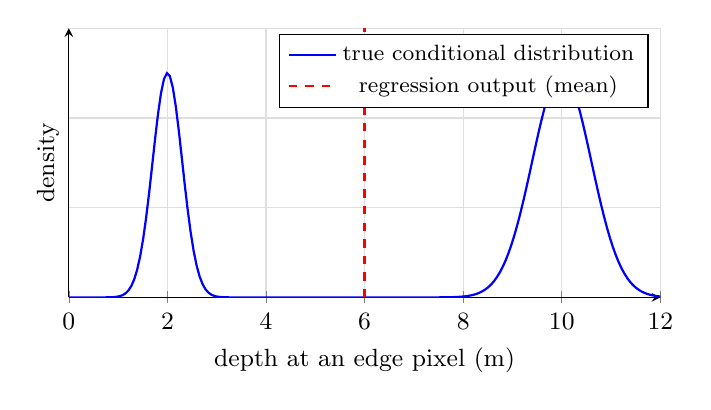
\begin{tikzpicture}
\begin{axis}[width=0.75\linewidth,height=5cm,domain=0:12,samples=200,axis lines=left,
  xlabel={depth at an edge pixel (m)},ylabel={density},ymajorticks=false,
  legend style={at={(0.98,0.98)},anchor=north east,font=\footnotesize}]
\addplot[thick,blue]{0.5*exp(-(x-2)^2/0.18)+0.5*exp(-(x-10)^2/0.72)};
\addplot[thick,red,dashed,samples=2] coordinates {(6,0)(6,0.6)};
\legend{true conditional distribution,regression output (mean)}
\end{axis}
\end{tikzpicture}
\caption{Original toy figure: a bimodal conditional distribution at a depth edge. The regressor answers the mean, which lies in a gap where the density is zero; a generative model can return a sample from one of the two modes.}
\end{figure}

\subsection{Many Outputs for One Input -- Text to Image \slides{10}}
One conditioning input has many valid completions. A regressor averages them; a diffusion model picks one.

\begin{figure}[H]
	\centering
	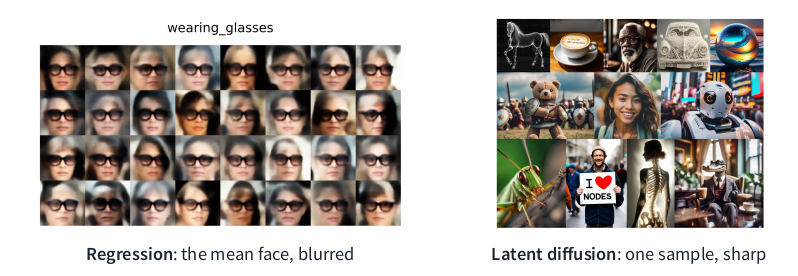
\includegraphics[width=1.0\linewidth]{1790765807667.png}
	\caption{left: grid of ``wearing\_glasses'' faces from regression (the mean face, blurred); right: grid of latent-diffusion samples (one sample, sharp)}\label{fig:1790765807667}
\end{figure}

\begin{intuition}
Blur is not a training failure. It is the correct answer to the wrong question: the conditional mean of a set of sharp images is not a sharp image. The same averaging is what flattens a depth edge.
\end{intuition}

\subsection{The Forward and Reverse Process \slides{11}}
The \textbf{forward process} adds noise to data one step at a time until nothing of the data is left. It is fixed and has no parameters. It is inspired by Brownian motion (many small independent displacements), and after enough steps the sample is indistinguishable from Gaussian noise. A diffusion model learns the \textbf{reverse process}, which recovers data from noise; that reverse process \emph{is the prior}.

\begin{definition}[Forward and reverse processes]
The forward chain $q(\bx_t\mid\bx_{t-1})$ maps $\bx_0$ (data) to $\bx_T$ (noise) and is fixed; the model $p_\theta(\bx_{t-1}\mid\bx_t)$ learns the way back.
\end{definition}

\begin{figure}[H]
\centering
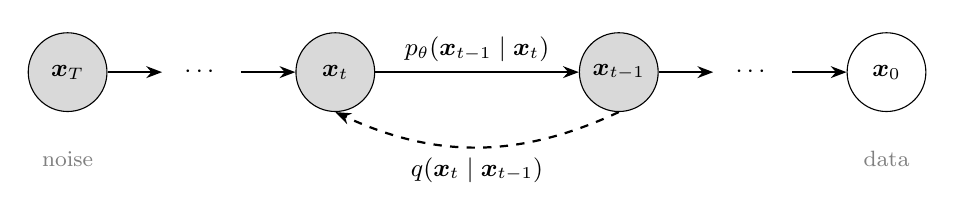
\begin{tikzpicture}[font=\small]
\node[draw,circle,fill=gray!30,minimum size=1cm] (xT) at (0,0){$\bx_T$};
\node at (1.7,0){$\cdots$};
\node[draw,circle,fill=gray!30,minimum size=1cm] (xt) at (3.4,0){$\bx_t$};
\node[draw,circle,fill=gray!30,minimum size=1cm] (xt1) at (7,0){$\bx_{t-1}$};
\node at (8.7,0){$\cdots$};
\node[draw,circle,minimum size=1cm] (x0) at (10.4,0){$\bx_0$};
\draw[arr] (xT)--(1.2,0); \draw[arr] (2.2,0)--(xt);
\draw[arr] (xt)--node[above]{$p_\theta(\bx_{t-1}\mid\bx_t)$}(xt1);
\draw[arr] (xt1)--(8.2,0); \draw[arr] (9.2,0)--(x0);
\draw[arr,dashed] (xt1.south) to[bend left=25] node[below]{$q(\bx_t\mid\bx_{t-1})$} (xt.south);
\node[font=\footnotesize,gray] at (0,-1.1){noise}; \node[font=\footnotesize,gray] at (10.4,-1.1){data};
\end{tikzpicture}
\caption{Forward (dashed, fixed) and reverse (solid, learned) chains, redrawn from slide 11.}
\end{figure}

\begin{figure}[H]
\centering
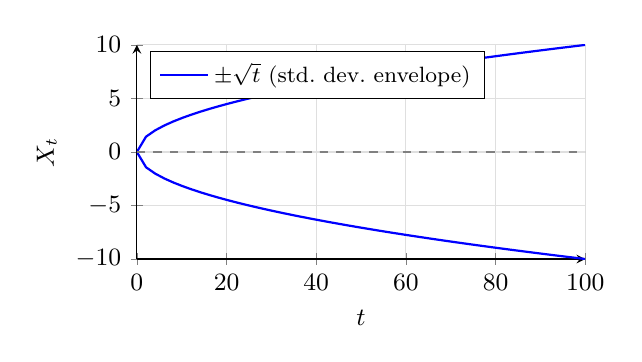
\begin{tikzpicture}
\begin{axis}[width=0.6\linewidth,height=4.3cm,domain=0:100,samples=50,axis lines=left,xlabel={$t$},ylabel={$X_t$},
  legend style={font=\footnotesize,at={(0.03,0.97)},anchor=north west}]
\addplot[thick,blue]{sqrt(x)}; \addplot[thick,blue]{-sqrt(x)}; \addplot[dashed,gray]{0};
\legend{$\pm\sqrt{t}$ (std.\ dev.\ envelope)}
\end{axis}
\end{tikzpicture}
\caption{Original figure: the spread of a random walk grows like $\sqrt t$, the mechanism that buries the data in noise.}
\end{figure}
\begin{figure}[H]
	\centering
	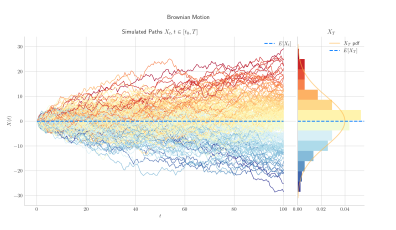
\includegraphics[width=1.0\linewidth]{1790765932964.png}
	\caption{Brownian-motion simulated paths (coloured bundle of trajectories) with the histogram of $X_T$ on the right, and the two small face images (noisy, clean) below the chain}\label{fig:1790765932964}
\end{figure}
\subsection{Training by Noise Prediction \slides{12}}
A denoising diffusion model estimates the noise vector $\beps$ from a noise level $\sigma>0$ and a noisy input $\bx_\sigma\approx\bx_0+\sigma\beps$, where $\bx_0$ lies on the data manifold $\mathcal{K}\subset\R^n$.

\begin{definition}[Denoiser and training loss]
A denoiser $\beps_\theta:\R^n\times\R_+\to\R^n$ is learned by minimizing
\begin{equation}\label{eq:lsimple}
L_{\text{simple}}(\theta):=\E_{\bx_0,\sigma,\beps}\Bigl[\bigl\|\beps_\theta(\bx_0+\sigma\beps,\sigma)-\beps\bigr\|^2\Bigr],
\end{equation}
with $\bx_0$ sampled from the training data, $\sigma$ from a training noise schedule, and $\beps\sim\mathcal N(\bm 0,\bm I)$.
\end{definition}

\begin{intuition}
The recipe is three lines: take a clean example, add noise of a random strength you remember, and ask the network ``what noise did I add?''. Subtracting the guessed noise gives the guessed clean point, $\hat\bx_0=\bx_\sigma-\sigma\beps_\theta$. No labels beyond the data itself are needed.
\end{intuition}

\subsection{The Spiral Toy Model \slides{13}}
Everything that follows is shown on a 2D data set, where the prior is visible: \emph{it is where the points are}. The data are points of a 2D spiral $\bx_0$. The network is a fully connected MLP fed with $\bx_0+\sigma\beps$ and a 2D noise-level embedding of $\sigma$, and it predicts the noise.

\begin{lstlisting}
def get_sigma_embeds(sigma):
    sigma = sigma.unsqueeze(1)
    return torch.cat([torch.sin(torch.log(sigma)/2),
                      torch.cos(torch.log(sigma)/2)], dim=1)

class TimeInputMLP(nn.Module):
    def __init__(self, dim, hidden_dims):
        super().__init__()
        layers = []
        for in_dim, out_dim in pairwise((dim + 2,) + hidden_dims):
            layers.extend([nn.Linear(in_dim, out_dim), nn.GELU()])
        layers.append(nn.Linear(hidden_dims[-1], dim))
        self.net = nn.Sequential(*layers)
        self.input_dims = (dim,)

    def forward(self, x, sigma):
        sigma_embeds = get_sigma_embeds(sigma)
        nn_input = torch.cat([x, sigma_embeds], dim=1)
        return self.net(nn_input)

model = TimeInputMLP(dim=2, hidden_dims=(16,128,128,128,128,16))
\end{lstlisting}

\begin{intuition}
The extra two inputs $(\sin,\cos)$ of $\log\sigma/2$ tell the network \emph{how noisy} its input is. This matters because the right answer depends on $\sigma$: at small $\sigma$ the noise is a small nudge off the nearest data point, at large $\sigma$ the input is almost pure noise. Note that the first layer has width $\text{dim}+2=4$: two coordinates plus the two embedding numbers.
\end{intuition}

\subsection{Training the Toy Model \slides{14}}
\begin{lstlisting}
def training_loop(loader, model, schedule, epochs=10000):
    optimizer = torch.optim.Adam(model.parameters())
    for _ in range(epochs):
        for x0 in loader:
            optimizer.zero_grad()
            sigma, eps = generate_train_sample(x0, schedule)
            eps_hat = model(x0 + sigma * eps, sigma)
            loss = nn.MSELoss()(eps_hat, eps)
            loss.backward()
            optimizer.step()
\end{lstlisting}
The learned denoiser can be drawn as a \textbf{vector field} by plotting $\bx-\sigma\beps_\theta(\bx,\sigma)$. \emph{At small noise the arrows point at the nearest data. At large noise they point at the middle of the whole data set.} The slide's training curve falls from about $0.70$ to about $0.41$ over 15\,000 epochs.

\begin{figure}[H]
\centering
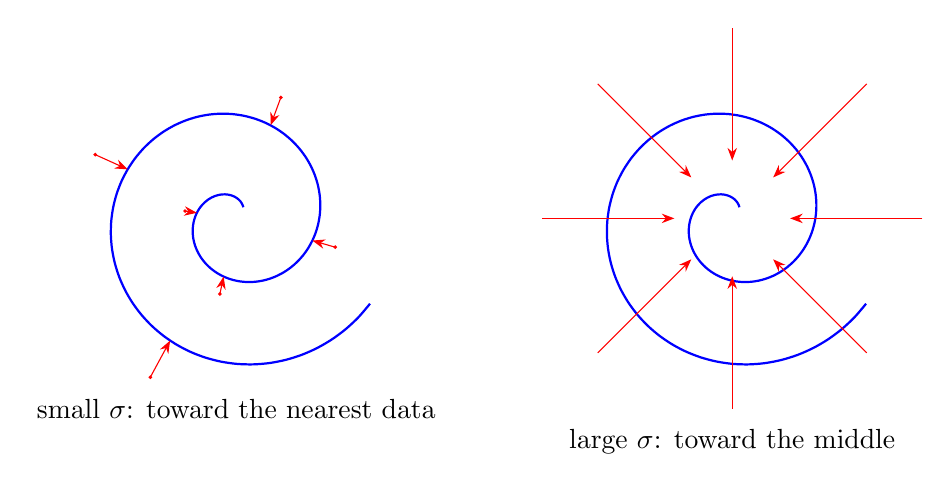
\begin{tikzpicture}[scale=2.1]
\begin{scope}
 \draw[blue,thick,domain=1:12,samples=100,smooth,variable=\t] plot ({0.08*\t*cos(\t r)},{0.08*\t*sin(\t r)});
 \foreach \t in {3,4.5,6,7.5,9,10.5}{
   \draw[-{Stealth[length=1.6mm]},red] ({1.3*0.08*\t*cos(\t r)},{1.3*0.08*\t*sin(\t r)})--({0.08*\t*cos(\t r)},{0.08*\t*sin(\t r)});
   \fill[red] ({1.3*0.08*\t*cos(\t r)},{1.3*0.08*\t*sin(\t r)}) circle (0.012);}
 \node at (0,-1.15) {small $\sigma$: toward the nearest data};
\end{scope}
\begin{scope}[xshift=3cm]
 \draw[blue,thick,domain=1:12,samples=100,smooth,variable=\t] plot ({0.08*\t*cos(\t r)},{0.08*\t*sin(\t r)});
 \foreach \a in {0,45,...,315}{\draw[-{Stealth[length=1.6mm]},red] (\a:1.15)--(\a:0.35);}
 \node at (0,-1.35) {large $\sigma$: toward the middle};
\end{scope}
\end{tikzpicture}
\caption{Original sketch of the denoiser field on the spiral (compare slide 14).}
\end{figure}

\begin{remark}[Why the loss does not reach zero]
The curve plateaus near $0.41$, not $0$. This is expected: even the best possible denoiser cannot recover $\beps$ exactly, because many $(\bx_0,\beps)$ pairs produce the same $\bx_\sigma$; the floor equals the average posterior variance of $\beps$ (Appendix~\ref{app:supp}, item~\ref{app:floor}).
\end{remark}

\subsection{The Ideal Denoiser \slides{15}}
The \textbf{ideal denoiser} minimizes the training loss; it is a function of the data set $\mathcal{K}$ and the noise level, and nothing else:
\begin{equation}
\beps^\ast:=\argmin_{\beps_\theta}\E_{\bx_0,\sigma,\beps}\bigl\|\beps_\theta(\bx_0+\sigma\beps,\sigma)-\beps\bigr\|^2 .
\end{equation}

\begin{theorem}[Ideal denoiser for a finite data set]\label{thm:ideal}
For a finite $\mathcal{K}$ (data uniformly distributed on $\mathcal{K}$, Gaussian noise),
\begin{equation}
\beps^\ast(\bx_\sigma,\sigma)=\frac{\sum_{\bx_0\in\mathcal{K}}(\bx_\sigma-\bx_0)\,\exp\!\bigl(-\|\bx_\sigma-\bx_0\|^2/2\sigma^2\bigr)}{\sigma\sum_{\bx_0\in\mathcal{K}}\exp\!\bigl(-\|\bx_\sigma-\bx_0\|^2/2\sigma^2\bigr)} .
\end{equation}
It is a weighted average of all data points: nearer points count more.
\end{theorem}
\begin{proof}
By the conditional-mean proposition, $\beps^\ast(\bx_\sigma,\sigma)=\E[\beps\mid\bx_\sigma]$ with $\beps=(\bx_\sigma-\bx_0)/\sigma$. By Bayes, $p(\bx_0\mid\bx_\sigma)\propto\exp(-\|\bx_\sigma-\bx_0\|^2/2\sigma^2)$ on $\mathcal{K}$. Taking the expectation of $(\bx_\sigma-\bx_0)/\sigma$ under these weights gives the formula.
\end{proof}

\begin{intuition}
Worked 1D example with $\mathcal{K}=\{-1,+1\}$, $\bx_\sigma=0.2$. For $\sigma=0.5$ the weights are $e^{-1.44/0.5}\approx0.056$ (for $-1$) and $e^{-0.64/0.5}\approx0.278$ (for $+1$), giving $\beps^\ast\approx-0.93$ and clean estimate $\hat\bx_0=0.2-0.5\cdot(-0.93)\approx0.66$: pulled toward the nearer point $+1$. For a large $\sigma=5$ the two weights are almost equal ($0.972$ vs $0.987$), $\beps^\ast\approx0.04$ and $\hat\bx_0\approx0.01$: the arrow points at the middle of the data set, exactly as in the slide's three panels ($\sigma=0.01,0.1,0.5$).
\end{intuition}

\subsection{The Smoothed Distance Function \slides{16}}
The distance to a set, $\mathrm{dist}_\mathcal{K}(\bx):=\inf\{\|\bx-\bx_0\|:\bx_0\in\mathcal{K}\}$, is not differentiable everywhere, so its gradient is hard to learn. Smoothing it by $\sigma$ fixes that.

\begin{definition}[Smoothed distance]
\begin{equation}
D_\sigma(\bx):=-\sigma^2\log\Bigl(\sum_{\bx_0\in\mathcal{K}}\exp\bigl(-\|\bx_0-\bx\|^2/2\sigma^2\bigr)\Bigr).
\end{equation}
(The slide denotes the smoothed squared distance by $\mathrm{dist}^2_\mathcal{K}(\bx,\sigma)$ and writes the identity below with a factor $\tfrac12$; with the definition as printed, $\tfrac12\mathrm{dist}^2_\mathcal{K}(\bx,\sigma)$ corresponds to $D_\sigma$.)
\end{definition}

\begin{proposition}[Denoiser = gradient of the smoothed distance]\label{prop:dist}
$\displaystyle \tfrac12\nabla_{\bx}\,\mathrm{dist}^2_\mathcal{K}(\bx,\sigma)=\nabla_{\bx}D_\sigma(\bx)=\sigma\,\beps^\ast(\bx,\sigma)$, and $\min_{\bx_0}\tfrac12\|\bx-\bx_0\|^2-\sigma^2\log|\mathcal{K}|\le D_\sigma(\bx)\le\min_{\bx_0}\tfrac12\|\bx-\bx_0\|^2$.
\end{proposition}
\begin{proof}
Differentiating, $\nabla D_\sigma=-\sigma^2\cdot\frac{\sum e^{-\|\bx_0-\bx\|^2/2\sigma^2}\,(-(\bx-\bx_0)/\sigma^2)}{\sum e^{-\|\bx_0-\bx\|^2/2\sigma^2}}=\frac{\sum(\bx-\bx_0)e^{\cdots}}{\sum e^{\cdots}}=\sigma\beps^\ast$ by Theorem~\ref{thm:ideal}. The bounds follow from $e^{-a_{\min}/\sigma^2}\le\sum_i e^{-a_i/\sigma^2}\le|\mathcal{K}|\,e^{-a_{\min}/\sigma^2}$ with $a_i=\tfrac12\|\bx-\bx_{0,i}\|^2$.
\end{proof}

\begin{figure}[H]
	\centering
	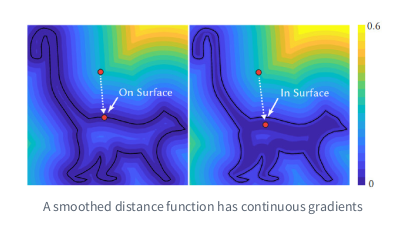
\includegraphics[width=1.0\linewidth]{1790765980671.png}
	\caption{the two coloured distance-field images of the cat silhouette (``On Surface'' and ``In Surface'' with the dotted arrows), with the colour bar 0--0.6}\label{fig:1790765980671}
\end{figure}

\begin{intuition}
$\min$ has kinks where two data points are equally near; a \emph{soft}-min has none, and its slope is the vector from the weighted mean of the data to $\bx$. So the denoiser is a compass that is defined \emph{everywhere} and always points toward the data: that is what makes it a prior. Equivalently $\hat\bx_0=\bx_\sigma-\sigma\beps^\ast$ is simply the weighted mean of the data points.
\end{intuition}

\subsection{Sampling From a Diffusion Model -- Why iterative? \slides{17}}
Given a noisy $\bx_\sigma$ and its noise level, the denoiser estimates the clean point directly,
\begin{equation}
\hat\bx_0(\bx_\sigma,\sigma):=\bx_\sigma-\sigma\beps_\theta(\bx_\sigma,\sigma).
\end{equation}
A sampler walks a decreasing sequence of noise levels, taking one such estimate at each step. \textbf{DDIM} is the update
\begin{equation}\label{eq:ddim}
\bx_{t-1}=\bx_t+(\sigma_{t-1}-\sigma_t)\,\beps_\theta(\bx_t,\sigma_t).
\end{equation}

\begin{figure}[H]
\centering
\begin{tikzpicture}[font=\small]
\draw[green!50!black,thick] (0,0) .. controls (-0.6,1.3) and (1.6,2.0) .. (2.1,0.9) .. controls (2.7,-0.3) and (1,-1) .. (0,0);
\node[green!50!black] at (0.8,0.7){$\mathcal{K}$};
\coordinate (xt) at (7,3.8); \coordinate (x0h) at (1.3,0.1);
\coordinate (xt1) at ($(xt)!0.28!(x0h)$);
\fill (xt) circle (2pt) node[above right]{$\bx_t$};
\fill (xt1) circle (2pt) node[left]{$\bx_{t-1}$};
\fill (x0h) circle (2pt) node[below]{$\hat\bx_0^{\,t}$};
\draw[dotted,blue,thick] (xt1)--(x0h);
\draw[arr,blue] (xt)--(xt1) node[midway,above left]{$(\sigma_{t-1}-\sigma_t)\,\beps_\theta(\bx_t)$};
\end{tikzpicture}
\caption{DDIM step (redrawn from slide 17): a straight line toward the current estimate $\hat\bx_0^{\,t}$ of the data.}
\end{figure}

\begin{intuition}
One step goes only \emph{part} of the way to the current best guess, because the guess is poor while the input is very noisy; after moving, you re-evaluate the compass. The step is a straight line toward the estimate. This is the equation that depth completion reaches inside and steers (Section~\ref{sec:dc}). Algebraically the step re-noises the clean estimate to the lower level: $\bx_{t-1}=\hat\bx_0^{\,t}+\sigma_{t-1}\beps_\theta$ (Appendix~\ref{app:supp}).
\end{intuition}

\subsection{The DDIM Sampler \slides{18}}
\begin{algorithm}[DDIM sampler]\label{alg:ddim}
\texttt{for t = N, ..., 1:} \quad $\bx_{t-1}\leftarrow\bx_t+(\sigma_{t-1}-\sigma_t)\,\beps_\theta(\bx_t,\sigma_t)$; \quad \texttt{return} $\bx_0$. \\
Start from $\bx_N=\sigma_N\cdot\mathcal N(\bm0,\bm I)$.
\end{algorithm}
\begin{lstlisting}
@torch.no_grad()
def samples_ddim(model, sigmas, batchsize=1):
    xt = model.rand_input(batchsize) * sigmas[0]
    for sig, sig_prev in pairwise(sigmas):
        xt = xt - (sig - sig_prev) * model.predict_eps(xt, sig)
    return xt
\end{lstlisting}
On the toy model: \emph{fifty steps, no retraining, and the trajectory follows the field.}

\subsection{Probabilistic Sampling \slides{19}}
DDIM is deterministic: the same starting noise always gives the same sample. Adding a noise term back makes the sampler stochastic:
\begin{equation}
\bx_{t-1}=\bx_t+(\sigma_{t-1}-\sigma_t)\,\beps_\theta(\bx_t,\sigma_t)+\mu\,\bm w_t,\qquad \bm w_t\sim\mathcal N(\bm0,\bm I).
\end{equation}
(The slide writes $\sigma_{t'}$ for the next, lower level.) With $\mu=0$ this is DDIM again; as $\mu$ grows the trajectories spread, and the same input gives different samples. The slide shows $\mu=0.001,0.01,0.1$.

\begin{intuition}
$\mu$ is a ``temperature'': $\mu=0$ rolls a ball down a fixed groove, $\mu>0$ shakes the table on the way. This is the reason different seeds give different depth maps in Marigold (Section~\ref{sec:marigold}).
\end{intuition}

\subsection{Three Uses of a Prior \slides{20}}
A prior that exists as a \textbf{separate object} can be used in three ways, each a later section of the lecture.
\begin{center}\small
\begin{tabular}{@{}p{2.2cm}p{7cm}l@{}}\toprule
use & meaning & section\\\midrule
\textbf{Sample} & draw from the distribution the model represents & 3.10\\
\textbf{Condition} & train it with a side input $\bm c$, so it samples from $\mathrm p(\bx\mid\bm c)$ & 3.11\\
\textbf{Guide} & modify the state inside the sampling loop at test time, with no retraining & 3.13\\\bottomrule
\end{tabular}
\end{center}
The third is the one that turns a depth prior into a metric depth map.

\begin{figure}[H]
	\centering
	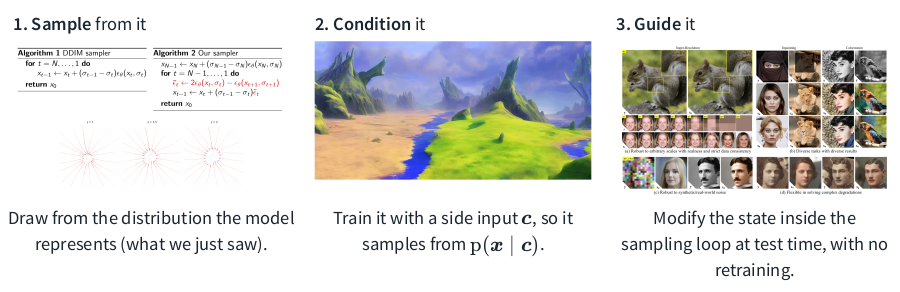
\includegraphics[width=1.0\linewidth]{1790766095193.png}
	\caption{the three panels: sampler comparison plots (Algorithm 1 vs Algorithm 2), the generated landscape (conditioning), and the super-resolution / inpainting / colorization examples (guidance)}\label{fig:1790766095193}
\end{figure}

\subsection{The Autoencoder and Latent Diffusion \slides{21}}
Images are big, so an autoencoder compresses them first: an encoder $\mathcal E$ maps $\bx$ to a latent $\bz$, and a decoder $\mathcal D$ maps back, $\bz=\mathcal E(\bx)$, $\tilde\bx=\mathcal D(\bz)$. The autoencoder is trained \textbf{first}, then \textbf{frozen}; the diffusion model never sees pixels and you decode once, at the end. Diffusion runs on $\bz$ with the same loss:
\begin{equation}
L=\E_{\sigma,\bz_0,\beps}\Bigl[\bigl\|\beps-\beps_\theta(\bz_0+\sigma\beps,\sigma)\bigr\|^2\Bigr].
\end{equation}

\begin{figure}[H]
\centering
\resizebox{\linewidth}{!}{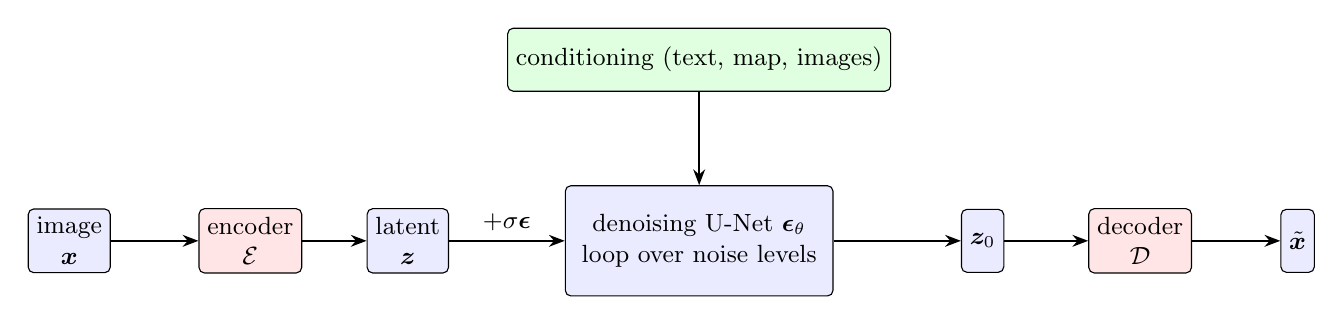
\begin{tikzpicture}[font=\small]
\node[box] (x) at (0,0){image\\$\bx$};
\node[frozen] (E) at (2.3,0){encoder\\$\mathcal E$};
\node[box] (z) at (4.3,0){latent\\$\bz$};
\node[box,minimum width=3.4cm,minimum height=1.4cm] (u) at (8,0){denoising U-Net $\beps_\theta$\\loop over noise levels};
\node[box] (z0) at (11.6,0){$\bz_0$};
\node[frozen] (D) at (13.6,0){decoder\\$\mathcal D$};
\node[box] (xt) at (15.6,0){$\tilde\bx$};
\node[box,fill=green!12] (c) at (8,2.3){conditioning (text, map, images)};
\draw[arr] (x)--(E); \draw[arr] (E)--(z); \draw[arr] (z)--node[above]{$+\sigma\beps$}(u);
\draw[arr] (u)--(z0); \draw[arr] (z0)--(D); \draw[arr] (D)--(xt); \draw[arr] (c)--(u);
\end{tikzpicture}}
\caption{Latent diffusion in outline (original, inspired by slide 21). Pink boxes are frozen autoencoder parts.}
\end{figure}

\begin{intuition}
Worked numbers: $768\times768\times3\to96\times96\times4$, i.e. $1\,769\,472$ numbers become $36\,864$: eight times smaller per side, four channels, \textbf{48 times fewer numbers}. Each of the 50 denoising steps is therefore 48 times cheaper than it would be in pixel space.
\end{intuition}

\subsection{Conditioning and Guidance \slides{22}}
\textbf{Conditioning} is a side input the network was \emph{trained with}; the model responds to it because it was trained to. \textbf{Guidance} modifies the sampling trajectory \emph{at test time}, using a criterion the network was never trained on. Sampling is a loop, and its state can be modified between steps.

\begin{figure}[H]
\centering
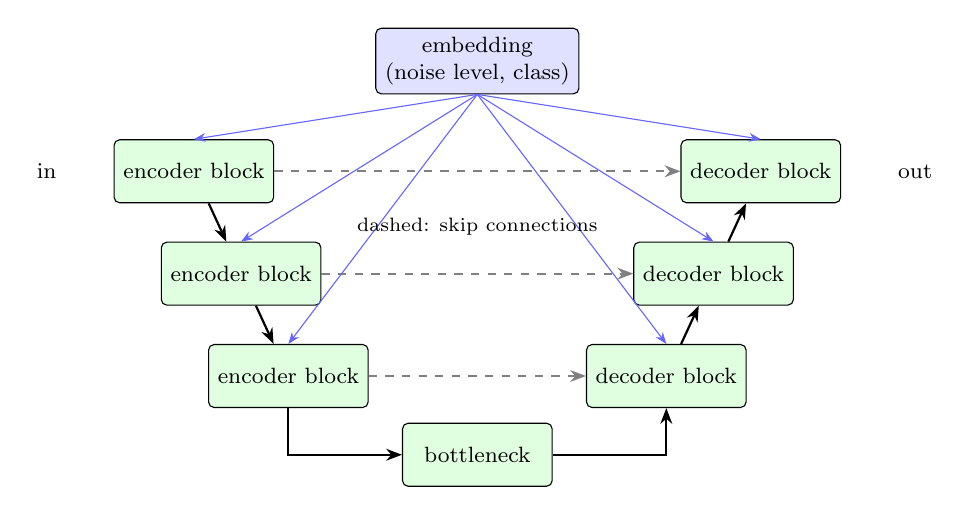
\begin{tikzpicture}[font=\footnotesize,
  blk/.style={draw,fill=green!12,minimum width=1.9cm,minimum height=0.8cm,align=center,rounded corners=2pt}]
\node[blk,fill=blue!12] (emb) at (3.6,4.4){embedding\\(noise level, class)};
\node[blk] (e1) at (0,3){encoder block};
\node[blk] (e2) at (0.6,1.7){encoder block};
\node[blk] (e3) at (1.2,0.4){encoder block};
\node[blk] (m) at (3.6,-0.6){bottleneck};
\node[blk] (d3) at (6,0.4){decoder block};
\node[blk] (d2) at (6.6,1.7){decoder block};
\node[blk] (d1) at (7.2,3){decoder block};
\draw[arr] (e1)--(e2); \draw[arr] (e2)--(e3); \draw[arr] (e3)|-(m); \draw[arr] (m)-|(d3);
\draw[arr] (d3)--(d2); \draw[arr] (d2)--(d1);
\draw[arr,dashed,gray] (e1)--(d1); \draw[arr,dashed,gray] (e2)--(d2); \draw[arr,dashed,gray] (e3)--(d3);
\foreach \n in {e1,e2,e3,d1,d2,d3}{\draw[-{Stealth[length=1.5mm]},blue!60] (emb.south)--(\n.north);}
\node[left=0.6cm of e1]{in}; \node[right=0.6cm of d1]{out};
\node[font=\scriptsize,align=center] at (3.6,2.3){dashed: skip connections};
\end{tikzpicture}
\caption{Simplified U-Net redrawn from slide 22. Each block is GroupNorm--SiLU--Conv$3{\times}3$ with the embedding injected through a Linear layer (scale and shift); attention is optional.}
\end{figure}

%=====================================================================
\section{Marigold \slides{23--31}}\label{sec:marigold}
%=====================================================================
Section 3.11: a depth estimator from an image diffusion model. Stable Diffusion's autoencoder is kept, only its denoiser is fine-tuned, and the output is a depth map rather than an image.

\subsection{The Marigold Method \slides{24}}
\emph{The argument:} a monocular estimator's knowledge of the visual world is \textbf{bounded by its training set}, while a text-to-image model trained on billions of captioned photographs has already seen it. Hence: if the cornerstone of monocular depth is a comprehensive representation of the visual world, one should be able to derive a depth estimator from a pretrained image diffusion model.

\begin{definition}[Marigold]
Take a pretrained text-to-image latent diffusion model, \textbf{freeze the VAE}, and fine-tune only the denoising U-Net so that what it denoises is a \emph{depth} latent rather than an image latent. Properties from the slide: affine-invariant monocular depth; trained on \textbf{synthetic data only}; about 2.5 days on a single consumer GPU.
\end{definition}

\begin{figure}[H]
	\centering
	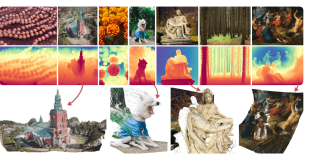
\includegraphics[width=1.0\linewidth]{1790766180369.png}
	\caption{the strip of example results: photographs (beads, church, marigolds, dog, sculpture, forest, painting) with their depth maps and back-projected 3D views}\label{fig:1790766180369}
\end{figure}

\subsection{From the Spiral to Marigold \slides{25}}
Marigold is the spiral model with one extra input; nothing in the algorithm changes.
\begin{center}\small
\begin{tabular}{@{}p{2.6cm}p{3.4cm}p{5.6cm}@{}}\toprule
 & toy model & Marigold\\\midrule
starts from & random weights & Stable Diffusion's weights\\
a data point & a 2D point & a depth latent\\
the denoiser & a small MLP & Stable Diffusion's U-Net\\
the condition & none & the image latent\\
trained on & spiral points & 74K rendered image--depth pairs\\
the sampler & DDIM & the same DDIM\\
a sample is & a point on the spiral & a depth map the RGB allows\\\bottomrule
\end{tabular}
\end{center}
The first row is the whole bet: \emph{the visual prior is already in those weights}, and fine-tuning moves what they denoise from images to depth. (Stable Diffusion indexes noise levels by a timestep $t$ and scales its input; both are fixed functions of $\sigma$, so the process is the same.)

\subsection{The Source of Affine Invariance \slides{26}}
The normalization defines the output space: the affine-invariant \emph{depth} row of the table in Part~I, not the affine-invariant \emph{disparity} row that MiDaS uses.

\begin{definition}[Percentile normalization]
With $\bm D_2$ and $\bm D_{98}$ the 2nd and 98th percentiles of the depth map $\bm D$, the training target is
\begin{equation}
\tilde{\bm D}=\Bigl(\frac{\bm D-\bm D_2}{\bm D_{98}-\bm D_2}-0.5\Bigr)\times2,\qquad\text{and metric depth is recovered as}\qquad \tilde{\bm D}_{\text{metric}}=s\tilde{\bm D}+t .
\end{equation}
\end{definition}

\begin{proposition}[Normalization removes scale and shift]
If $\bm D'=a\bm D+b$ with $a>0$, then $\tilde{\bm D}'=\tilde{\bm D}$.
\end{proposition}
\begin{proof}
Percentiles commute with increasing affine maps: $\bm D'_2=a\bm D_2+b$, $\bm D'_{98}=a\bm D_{98}+b$. Hence $(\bm D'-\bm D'_2)/(\bm D'_{98}-\bm D'_2)=a(\bm D-\bm D_2)/(a(\bm D_{98}-\bm D_2))$, the same ratio.
\end{proof}

\begin{figure}[H]
\centering
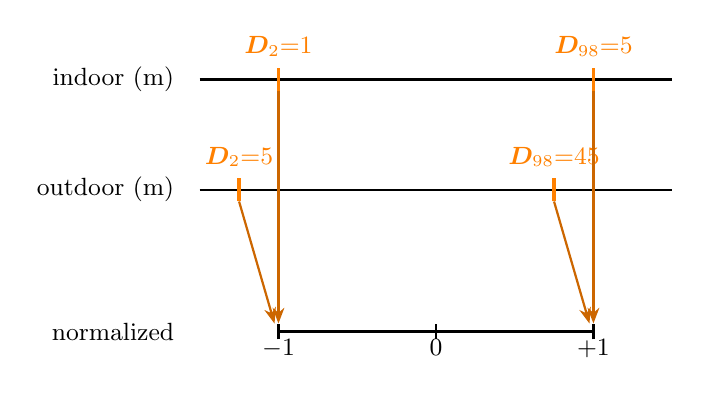
\begin{tikzpicture}[font=\small]
\draw[thick] (0,2.2)--(6,2.2); \node[anchor=east] at (-0.2,2.2){indoor (m)};
\draw[thick] (0,0.8)--(6,0.8); \node[anchor=east] at (-0.2,0.8){outdoor (m)};
\draw[thick] (1,-1)--(5,-1); \node[anchor=east] at (-0.2,-1){normalized};
\foreach \x/\l in {1/{$\bm D_2{=}1$},5/{$\bm D_{98}{=}5$}}{\draw[orange,very thick] (\x,2.05)--(\x,2.35) node[above]{\l};}
\foreach \x/\l in {0.5/{$\bm D_2{=}5$},4.5/{$\bm D_{98}{=}45$}}{\draw[orange,very thick] (\x,0.65)--(\x,0.95) node[above]{\l};}
\foreach \x/\l in {1/$-1$,3/$0$,5/$+1$}{\draw[thick] (\x,-1.1)--(\x,-0.9) node[below=2pt]{\l};}
\draw[arr,orange!80!black] (1,2.05)--(1,-0.9); \draw[arr,orange!80!black] (5,2.05)--(5,-0.9);
\draw[arr,orange!80!black] (0.5,0.65)--(0.95,-0.9); \draw[arr,orange!80!black] (4.5,0.65)--(4.95,-0.9);
\end{tikzpicture}
\caption{Original figure: an indoor map (few meters) and an outdoor map (tens of meters) land on the same $[-1,+1]$ range; each map is normalized by its \emph{own} percentiles (slide 26). The numbers are illustrative.}
\end{figure}

\begin{intuition}
Every training map is stretched to fill $[-1,+1]$, so a room and a highway look identical to the network in terms of range. \textbf{The model never sees meters and never sees a common zero, so it cannot learn them; it is constrained to predict shape.} Example: in a room with $\bm D_2=1$~m and $\bm D_{98}=5$~m, a pixel at $3$~m maps to $0$; on a street with $\bm D_2=5$~m and $\bm D_{98}=45$~m, a pixel at $25$~m also maps to $0$.
\end{intuition}

\subsection{Conditioning on the Image \slides{27}}
The denoiser takes the noisy depth latent $\bz^{(\bm D)}_\sigma$ and the image latent $\bz^{(\bm I)}$:
\begin{equation}
\beps_\theta\bigl(\bz^{(\bm D)}_\sigma,\,\bz^{(\bm I)},\,\sigma\bigr),\qquad \bz_\sigma=\mathrm{cat}\bigl(\bz^{(\bm D)}_\sigma,\bz^{(\bm I)}\bigr).
\end{equation}
The depth map is replicated to three channels and encoded by the \textbf{frozen RGB autoencoder}, whose reconstruction error on depth is negligible. \textbf{Concatenation} suits a condition that is spatially aligned with the output, pixel for pixel; cross-attention is for conditions that are not.

\begin{definition}[Four changes to the network]
(1) Concatenate the image latent and the noisy depth latent along the channels; (2) double the U-Net's input channels; (3) duplicate the first layer's weights and \textbf{halve} them, so activation magnitudes do not inflate; (4) \textbf{disable text conditioning} (original Stable Diffusion).
\end{definition}

\begin{intuition}
Why halve? Let the original first layer be $W\bz$. The new layer sees $[\bz;\bz]$ and uses $[W/2,\;W/2]$, so its output is $W\bz/2+W\bz/2=W\bz$: at the start of fine-tuning the pretrained network behaves as before. Without halving, the same input would produce $2W\bz$, twice the activations the pretrained weights expect. Since the latent has $4$ channels, the new input has $8$. Concatenation works here because the depth map and the image are aligned pixel by pixel.
\end{intuition}

\subsection{Training Marigold \slides{28}}
\begin{lstlisting}
def training_loop(loader, unet, vae, schedule, epochs):
    optimizer = torch.optim.Adam(unet.parameters())
    for _ in range(epochs):
        for image, depth in loader:                  # pairs
            optimizer.zero_grad()
            # start lock
            x0 = vae.encode(normalize(depth))        # a depth latent
            cond = vae.encode(image)                 # the condition
            # end lock
            sigma, eps = generate_train_sample(x0, schedule)
            eps_hat = unet(x0 + sigma*eps, cond, sigma)   # sees both
            loss = nn.MSELoss()(eps_hat, eps)
            loss.backward()
            optimizer.step()
\end{lstlisting}
The objective is the one from the spiral, unchanged. Only the U-Net trains; the VAE is frozen at both ends. Data: 74K rendered pairs, about 2.5 days on one consumer GPU.

\begin{figure}[H]
	\centering
	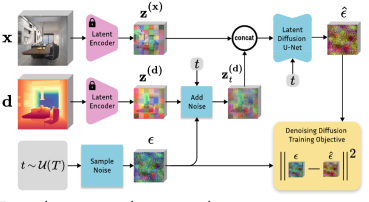
\includegraphics[width=1.0\linewidth]{1790766342627.png}
	\caption{Marigold training (redrawn from slides 27--28). Pink: frozen. The noise $\beps$ is also fed to the loss.}
\end{figure}

\subsection{Inference \slides{29}}
\begin{algorithm}[Marigold inference, one run]
(1) Encode the image \textbf{once}; (2) initialize the depth latent $\bz_T^{(\bm D)}$ as pure Gaussian noise; (3) run the denoising loop, concatenating the image latent at \textbf{every} step; (4) decode $\bz_0^{(\bm D)}$ and average the three channels. From the paper: 50 DDIM steps.
\end{algorithm}

\begin{figure}[H]
	\centering
	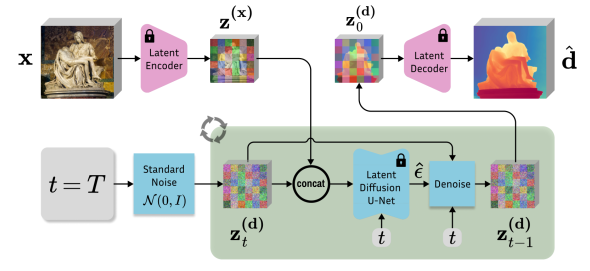
\includegraphics[width=1.0\linewidth]{1790766380221.png}
	\caption{Marigold inference}\label{fig:1790766380221}
\end{figure}

\subsection{Ensembling Over Samples \slides{30}}
Probabilistic sampling is why different seeds give different depth maps; Marigold runs the loop $N$ times and combines the results.
\begin{algorithm}[Ensembling]
(1) Each run is affine-invariant on its own scale, so first fit a scale and a shift per run so that the maps agree with each other (minimize the pairwise distance between the aligned maps, with a penalty that keeps the range on $[0,1]$); (2) take the pixel-wise \textbf{median}. Default $N=10$; \textbf{no ground truth is used}.
\end{algorithm}
\begin{intuition}
Ten drafts of the same drawing, each in its own unknown units. First rescale and shift each draft to line up with the others (they only agree up to $(s_i,t_i)$), then let the median vote at each pixel, which ignores outlier drafts.
\end{intuition}

\subsection{Limitations of Marigold \slides{31}}
\begin{itemize}[nosep]
 \item \textbf{No metric scale.}
 \item \textbf{No zero}: not even a common origin between two images of the same room.
 \item \textbf{Slow}: 50 denoising steps $\times$ 10 ensemble members $=500$ network evaluations per image.
 \item \textbf{It returns a sample} (non-deterministic).
\end{itemize}

%=====================================================================
\section{Back to 3D \slides{32--34}}
%=====================================================================
Section 3.12: back-projection turns a depth map into points and shows which of the unknown parameters distort the result.

\subsection{Effect of Scale and Shift Errors \slides{33}}
A depth map is a 2.5D surface: one depth per pixel, with nothing behind what is visible.

\begin{definition}[Back-projection]
\sloppy
\hbadness=10000
A pixel with intrinsics-normalized ray $\bm r=\bm K^{-1}(u,v,1)^\top$ and depth $z$ back-projects to $\bm p=z\,\bm r$.
\end{definition}

\begin{proposition}[Affine depth error]\label{prop:affine}
If $\hat z=sz+t$, the reconstructed point is $\hat{\bm p}=(s+t/z)\,\bm p$. In particular: the \textbf{scale} $s$ multiplies the whole cloud (a similarity, so shape is preserved); the \textbf{shift} $t$ drags every point a constant depth along its own ray, a different displacement in every direction (the shape can distort).
\end{proposition}
\begin{proof}
$\hat{\bm p}=\hat z\,\bm r=(sz+t)\bm r=(s+t/z)\,z\bm r$.
\end{proof}

\begin{corollary}[Affine error in disparity]
If disparity is $\hat d=sd+t$ then $\hat z=1/\hat d$ and $\hat{\bm p}=\bm p/(s+tz)$: a \emph{projective} map of space.
\end{corollary}
\begin{proof}
$\hat z=\dfrac{1}{s/z+t}=\dfrac{z}{s+tz}$, so $\hat{\bm p}=\hat z\bm r=\bm p/(s+tz)$.
\end{proof}

\begin{figure}[H]
\centering
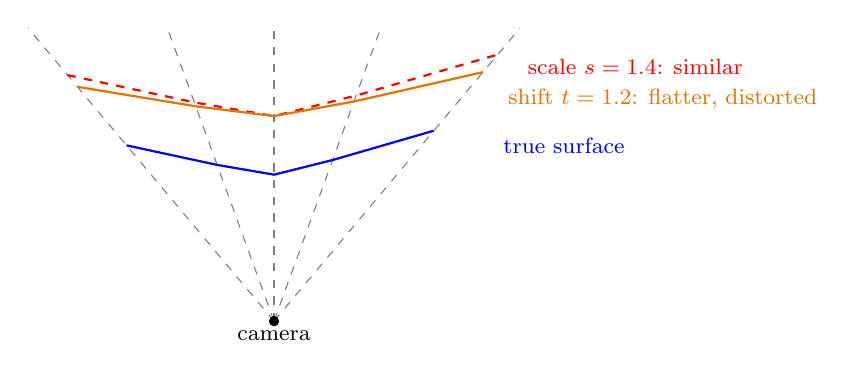
\begin{tikzpicture}[scale=0.62,font=\footnotesize]
\foreach \th in {-40,-20,0,20,40}{\draw[gray,dashed] (0,0)--({6*tan(\th)},6);}
\fill (0,0) circle (3pt) node[below]{camera};
\draw[blue,thick] (-3.02,3.6)--(-1.165,3.2)--(0,3.0)--(1.2,3.3)--(3.27,3.9);
\draw[red,thick,dashed] (-4.23,5.04)--(-1.63,4.48)--(0,4.2)--(1.68,4.62)--(4.58,5.46);
\draw[orange!90!black,thick] (-4.03,4.8)--(-1.6,4.4)--(0,4.2)--(1.64,4.5)--(4.28,5.1);
\node[blue,anchor=west] at (4.5,3.6){true surface};
\node[red,anchor=west] at (5.0,5.2){scale $s=1.4$: similar};
\node[orange!90!black,anchor=west] at (4.6,4.55){shift $t=1.2$: flatter, distorted};
\end{tikzpicture}
\caption{Original side view. A bowl-shaped surface seen along five rays. Scaling by $s$ keeps the shape (red); adding a constant depth $t$ along each ray (orange) keeps the depth differences but widens the lateral spread, so the bowl becomes flatter.}
\end{figure}

\begin{intuition}
Scale is a photocopier enlargement: bigger, same shape. Shift is pushing every point straight away from the camera by the same distance: because rays fan out, far-off directions move sideways more than the centre, so straight things bend. Example: $s=1$, $t=1$~m: a point at $z=2$ is scaled by $1+1/2=1.5$, one at $z=10$ by only $1.1$; near points are magnified more, so a wall receding from the camera is bent.
\end{intuition}

\subsection{Sources of Scale and Shift \slides{34}}
Two numbers are required, and a single image cannot supply them. Possible sources:
\begin{itemize}[nosep]
 \item a \textbf{metric-depth model}; camera-aware models narrow the generalization gap by taking the intrinsics as input (3.8);
 \item a \textbf{known baseline} at training time (3.9);
 \item a \textbf{known object size}: the apparent-size cue, which needs recognition;
 \item \textbf{known camera height plus a flat-ground assumption}: the vertical-position cue, which needs flat ground;
 \item or a \textbf{handful of real depth measurements}.
\end{itemize}

%=====================================================================
\section{Marigold-DC \slides{35--38}}\label{sec:dc}
%=====================================================================
Section 3.13: guidance from sparse depth measurements. Nothing is retrained: the denoising loop is modified at test time to move the sample toward the available measurements.

\subsection{The Depth Completion Task \slides{36}}
\begin{definition}[Depth completion]
Depth completion upgrades sparse depth measurements into dense depth maps guided by a conventional image. The sparse points come from the LiDAR returns of Part~I, structure-from-motion landmarks, or a phone's depth sensor.
\end{definition}

\begin{figure}[H]
	\centering
	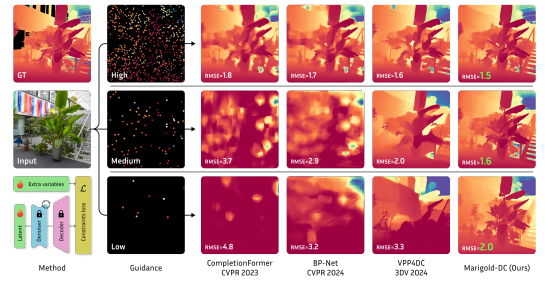
\includegraphics[width=1.0\linewidth]{1790766433535.png}
	\caption{the comparison grid: ground truth, input image and the sparse guidance at high / medium / low density, with the outputs of CompletionFormer, BP-Net, VPP4DC and Marigold-DC and their RMSE labels}\label{fig:1790766433535}
\end{figure}
\begin{center}\small
\begin{tabular}{@{}lcccc@{}}\toprule
guidance density & CompletionFormer & BP-Net & VPP4DC & Marigold-DC\\\midrule
high & 1.8 & 1.7 & 1.6 & \textbf{1.5}\\
medium & 3.7 & 2.9 & 2.0 & \textbf{1.6}\\
low & 4.8 & 3.2 & 3.3 & \textbf{2.0}\\\bottomrule
\end{tabular}\\[2pt]
RMSE values printed on slide 36 (units not stated on the slide).
\end{center}

\begin{figure}[H]
\centering
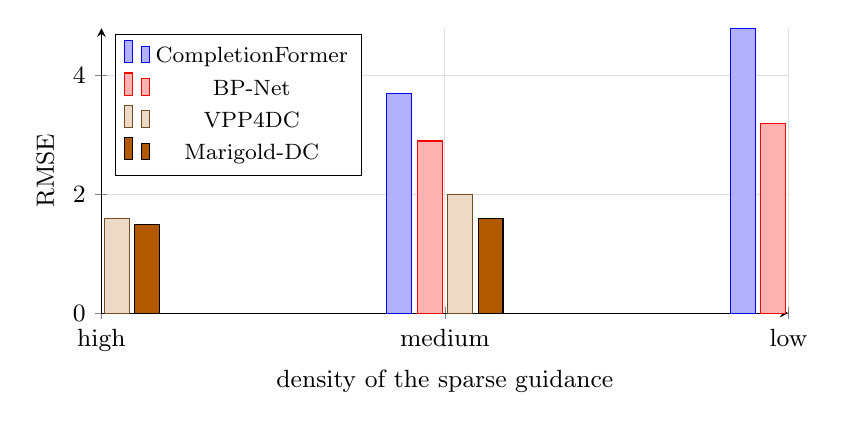
\begin{tikzpicture}
\begin{axis}[ybar,width=0.85\linewidth,height=5.2cm,bar width=9pt,ylabel={RMSE},symbolic x coords={high,medium,low},xtick=data,
  xlabel={density of the sparse guidance},ymin=0,enlarge x limits=0.25,legend style={font=\footnotesize,at={(0.02,0.98)},anchor=north west},axis lines=left]
\addplot coordinates {(high,1.8)(medium,3.7)(low,4.8)};
\addplot coordinates {(high,1.7)(medium,2.9)(low,3.2)};
\addplot coordinates {(high,1.6)(medium,2.0)(low,3.3)};
\addplot[fill=orange!70!black] coordinates {(high,1.5)(medium,1.6)(low,2.0)};
\legend{CompletionFormer,BP-Net,VPP4DC,Marigold-DC}
\end{axis}
\end{tikzpicture}
\caption{Plot of the RMSE numbers on slide 36. Baselines degrade quickly as the guidance gets sparser; Marigold-DC degrades slowly because the prior fills what the sensor did not sample.}
\end{figure}

\subsection{Steering the Loop \slides{37}}
Depth completion is reframed as \emph{image-conditional depth generation guided by sparse measurements}. It is \textbf{generation rather than regression}: the output comes from a prior. The image \textbf{conditions} the network, the sparse depth \textbf{guides} the loop, and the measurements were never part of training. Every step already walks toward the model's current estimate; a second pull is added, toward the measurements.

\begin{algorithm}[Guided step]
At every step of the loop:
(1) read the \emph{preview}, the current guess at the finished depth map, $\hat\bz_0^{\,t}=\bz_t-\sigma_t\beps_\theta$ (Tweedie formula);
(2) decode it and turn it into meters with the scale and the shift, $\hat{\bm d}^{(\mathrm m)}_t=\hat a\,\mathcal D(\hat\bz_0^{\,t})+\hat b$;
(3) compare it with the few pixels $\Omega$ that have a measurement $\bm c$, $\mathcal L=\bigl\|\hat{\bm d}^{(\mathrm m)}_t-\bm c\bigr\|_\Omega$;
(4) nudge the latent and the two scalars $(\hat a,\hat b)$ toward the measurements by gradient descent on $\mathcal L$;
(5) take the ordinary DDIM step.
\end{algorithm}

\begin{figure}[H]
\centering
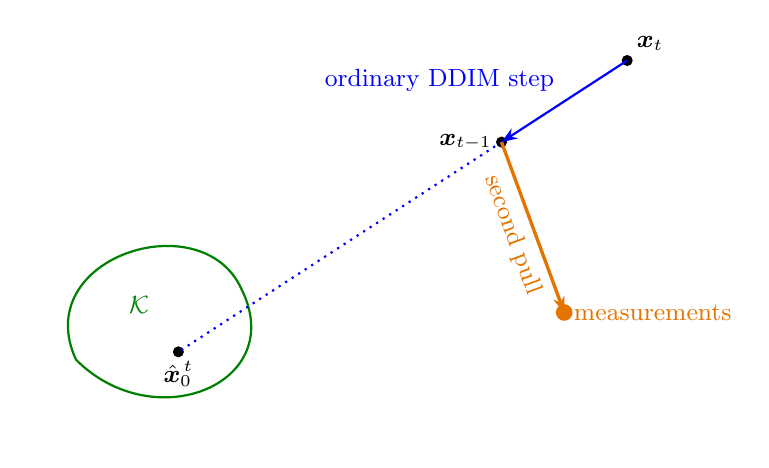
\begin{tikzpicture}[font=\small]
\draw[green!50!black,thick] (0,0) .. controls (-0.6,1.3) and (1.6,2.0) .. (2.1,0.9) .. controls (2.7,-0.3) and (1,-1) .. (0,0);
\node[green!50!black] at (0.8,0.7){$\mathcal{K}$};
\coordinate (xt) at (7,3.8); \coordinate (x0h) at (1.3,0.1);
\coordinate (xt1) at ($(xt)!0.28!(x0h)$);
\fill (xt) circle (2pt) node[above right]{$\bx_t$}; \fill (xt1) circle (2pt) node[left]{$\bx_{t-1}$};
\fill (x0h) circle (2pt) node[below]{$\hat\bx_0^{\,t}$};
\draw[dotted,blue,thick] (xt1)--(x0h);
\draw[arr,blue] (xt)--(xt1) node[midway,above left]{ordinary DDIM step};
\coordinate (M) at (6.2,0.6); \fill[orange!90!black] (M) circle (3pt) node[right]{measurements};
\draw[arr,orange!90!black,very thick] (xt1)--node[below,sloped]{second pull}(M);
\end{tikzpicture}
\caption{The guided step (redrawn from slide 37): DDIM step plus a second pull toward the sparse measurements.}
\end{figure}

\begin{figure}[H]
\centering
\resizebox{\linewidth}{!}{%
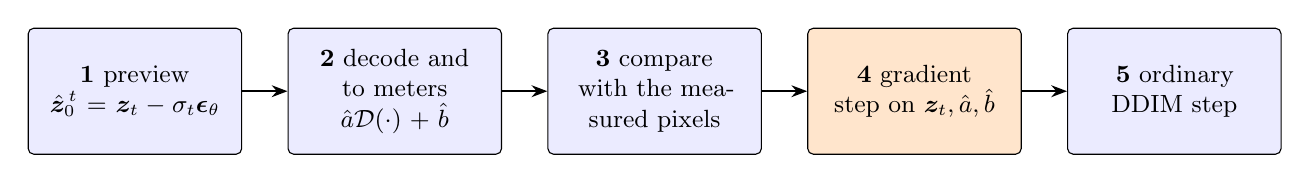
\begin{tikzpicture}[font=\small,st/.style={box,text width=2.5cm,minimum height=1.6cm}]
\node[st] (a) at (0,0){\textbf{1} preview\\$\hat\bz_0^{\,t}=\bz_t-\sigma_t\beps_\theta$};
\node[st] (b) at (3.3,0){\textbf{2} decode and to meters\\$\hat a\mathcal D(\cdot)+\hat b$};
\node[st] (c) at (6.6,0){\textbf{3} compare with the measured pixels};
\node[st,fill=orange!20] (d) at (9.9,0){\textbf{4} gradient step on $\bz_t,\hat a,\hat b$};
\node[st] (e) at (13.2,0){\textbf{5} ordinary DDIM step};
\foreach \p/\q in {a/b,b/c,c/d,d/e}{\draw[arr] (\p)--(\q);}
\end{tikzpicture}}
\caption{The five steps as a pipeline.}
\end{figure}

\subsection{Nothing Retrained \slides{38}}
Marigold gives affine-invariant depth; the sparse map gives \emph{metric} depth at a few pixels. The unknowns are the \textbf{latent}, which decides the shape, and the \textbf{scale and shift}, which decide the meters. All three are optimized, for one image, over fifty steps, and then discarded. Gradients are taken with respect to the latent and the two scalars, so \textbf{no weights change}: the U-Net and the VAE are frozen throughout.

\begin{theorem}[Zero-shot property, as claimed on the slide]
There is no depth-completion dataset, no architecture change and no new checkpoint. The method is therefore zero-shot across indoor and outdoor scenes, where the baselines ship one checkpoint per domain.
\end{theorem}

\begin{intuition}
The frozen network is a very good but unit-less sketch artist; the LiDAR points are a few tape-measure readings. At each step the sketch is bent slightly (through the latent) so that it does not contradict the readings, and the ruler (scale and shift) is adjusted until the sketch reads in meters. Because the readings are used only at test time, the same model handles a room and a street: the debts of Section~1 are paid at once, the prior supplying what the sensor cannot sample and the sensor the two numbers the prior cannot know.
\end{intuition}

\begin{figure}[H]
	\centering
	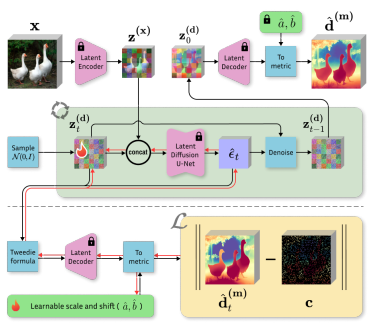
\includegraphics[width=1.0\linewidth]{1790766492486.png}
	\caption{the Marigold-DC diagram: goose photograph, encoder/decoder, frozen U-Net loop with the red gradient arrows, sparse map $\mathbf c$ and the resulting metric depth (the block structure is redrawn in the figures above)}\label{fig:1790766492486}
\end{figure}
% =====================================================================
\section*{Summary \slides{39--40}}
\addcontentsline{toc}{section}{Summary \emph{(slides 39--40)}}

\subsection*{Comparison of the methods covered}

\begin{center}
\scriptsize
\begin{tabularx}{\linewidth}{@{}>{\raggedright\arraybackslash}p{2.6cm}>{\raggedright\arraybackslash}p{1.9cm}>{\raggedright\arraybackslash}p{1.7cm}YY@{}}
\toprule
method & pays with & output & strength & main limitation\\
\midrule
Pulsed LiDAR & time & metric, sparse & exact where it lands; error nearly range-independent & stripes growing $\propto r$; no return $\neq0$; mixed points at edges\\
Rectified stereo & baseline & metric, dense where matched & dense; metric from $b$ & error $\propto z^2/(fb)$; fails on texture-poor, repeated, occluded regions\\
Structure from motion & computation & shape up to scale & no second camera needed & unknown global scale; rigid scene\\
Structured light (NYU) & projected pattern & metric, dense indoors & dense labels at short range & inpainted holes; indoor only\\
Geometric cues (size, vertical position) & assumptions & metric if assumptions hold & closed form, interpretable & need known $H$, flat ground, known $Y$ and horizon\\
Eigen scale-invariant loss & prior & depth up to 1 scale & loss respects scale ambiguity & one scale per scene; dataset-specific sensor errors\\
MiDaS & prior, mixed data & affine-invariant disparity & mixes datasets with no common zero & not metric; shape only\\
Depth Anything V2 & prior, pseudo-labels & affine-invariant inverse depth & scales with unlabeled real images & not metric without fine-tuning; inherits teacher's prior\\
\bottomrule
\end{tabularx}
\end{center}

\vspace{1em}
\noindent %=====================================================================
\emph{Every method in this lecture bought depth with a different resource. The last section bought it with two at once.}

\begin{center}\small
\begin{tabular}{@{}p{3.4cm}p{3.6cm}l p{4.2cm}@{}}\toprule
method & paid with & when & free parameters left\\\midrule
A laser (3.3, 3.4) & time & test & 0, but sparse\\
Stereo & a known baseline & test & 0, error grows as $z^2$\\
Structure from motion & viewpoints, no baseline & test & 1, one global scale\\
Supervised (3.7) & a prior, on sensor labels & train & 0, 1 or 2, set by the labels\\
Self-supervision (3.9) & a baseline & train & 0, for that rig\\
Marigold (3.11) & a generative prior & train & 2\\
Marigold-DC (3.13) & a prior and time & both & 0, dense, nothing retrained\\\bottomrule
\end{tabular}
\end{center}

\begin{figure}[H]
\centering
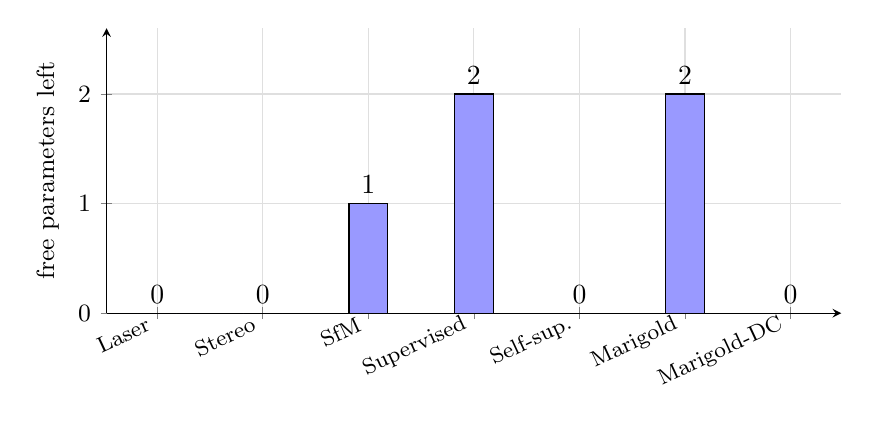
\begin{tikzpicture}
\begin{axis}[ybar,width=0.9\linewidth,height=5.2cm,bar width=14pt,symbolic x coords={Laser,Stereo,SfM,Supervised,Self-sup.,Marigold,Marigold-DC},
 xtick=data,xticklabel style={rotate=25,anchor=east,font=\footnotesize},ymin=0,ymax=2.6,ytick={0,1,2},ylabel={free parameters left},
 nodes near coords,axis lines=left,enlarge x limits=0.08]
\addplot[fill=blue!40] coordinates {(Laser,0)(Stereo,0)(SfM,1)(Supervised,2)(Self-sup.,0)(Marigold,2)(Marigold-DC,0)};
\end{axis}
\end{tikzpicture}
\caption{Free parameters left after each method (last column of the table). ``Supervised'' is drawn at its worst case: it ranges from 0 to 2 depending on the labels.}
\end{figure}

\subsection*{What each method lets you claim}

\begin{figure}[ht]
\centering
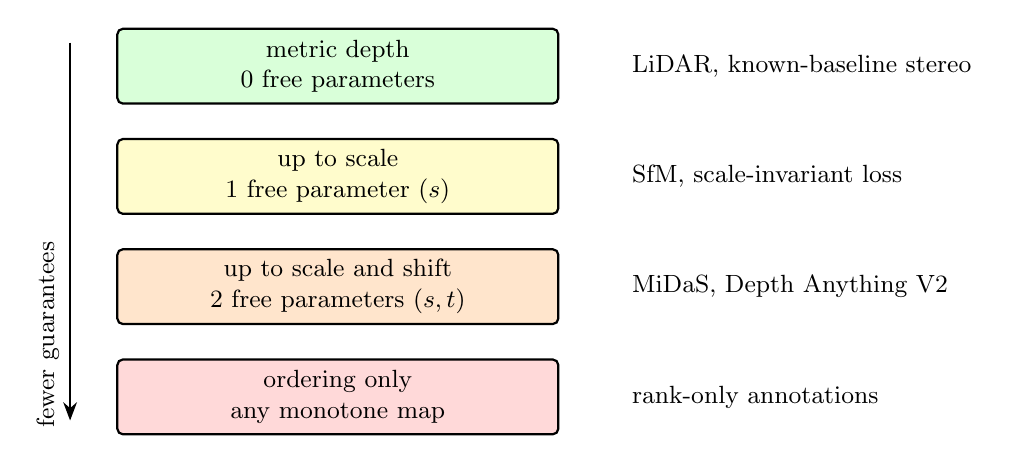
\begin{tikzpicture}[>=Stealth,
  lad/.style={draw,thick,rounded corners=2pt,minimum height=0.95cm,minimum width=5.6cm,align=center,font=\small}]
\node[lad,fill=green!15] (a) at (0,0) {metric depth\\ 0 free parameters};
\node[lad,fill=yellow!20] (b) at (0,-1.4) {up to scale\\ 1 free parameter ($s$)};
\node[lad,fill=orange!20] (c) at (0,-2.8) {up to scale and shift\\ 2 free parameters ($s,t$)};
\node[lad,fill=red!15] (d) at (0,-4.2) {ordering only\\ any monotone map};
\node[right=0.8cm of a,align=left,font=\small] {LiDAR, known-baseline stereo};
\node[right=0.8cm of b,align=left,font=\small] {SfM, scale-invariant loss};
\node[right=0.8cm of c,align=left,font=\small] {MiDaS, Depth Anything V2};
\node[right=0.8cm of d,align=left,font=\small] {rank-only annotations};
\draw[->,thick] (-3.4,0.3) -- (-3.4,-4.5) node[midway,left,rotate=90,font=\small,yshift=8pt]{fewer guarantees};
\end{tikzpicture}
\caption{Output spaces ordered by how much of the depth is actually determined. Moving down the ladder, the claim weakens but the data requirement does too.}
\end{figure}

\subsection*{Key take-aways}
\begin{itemize}
\item \textbf{Depth from one pixel is undetermined.} Back-projection returns a ray; metric depth always needs a \emph{currency}: time (LiDAR), a baseline (stereo) or a prior (learning). A single image bypasses cost, sparsity and hardware, but not the physics.
  \item \textbf{The two physical principles fail differently.} Time of flight has a range-independent timing floor but sparse, structured samples; triangulation is dense but its error grows as $z^2/(fb)$. LiDAR labels must be converted with the camera-frame $z$, a z-buffer and a validity mask.
  \item \textbf{A learned depth network is a prior, and its output is ambiguous.} The likelihood is flat along each ray, so scale-invariant and affine-invariant losses (in log space or in disparity) ask the network only for shape; disparity is preferred because planes stay planes under an affine map in inverse depth.
  \item \textbf{The prior is both the method and the failure mode.} Networks read vertical image position more than apparent size, only partially respect pitch and roll, and absorb the training focal length; anamorphic art defeats them with no sign of uncertainty.
  \item \textbf{Always ask ``recovered or ambiguous?''} Whether a reported depth is in meters, up to scale, or up to scale and shift determines what it can be used for (planning versus shape) and is the key to reading benchmark numbers (aligned first, then scored with AbsRel and $\delta$).
\item \textbf{The prior supplies what the sensor cannot sample, and the sensor supplies the two numbers the prior cannot know.}
 \item Self-supervision from stereo needs no depth labels, but the photometric loss is blind on flat and occluded pixels (hand-written priors fill the gap) and is metric only for the baseline it was trained with.
 \item A diffusion denoiser is a prior: it learns the gradient of a smoothed distance to the data, is defined everywhere, and can be sampled, conditioned, or guided; regression by contrast returns the conditional mean, which blurs depth edges.
 \item Marigold reuses Stable Diffusion's weights: frozen VAE, U-Net fine-tuned with the image latent concatenated; percentile normalization makes the output affine-invariant, so it gives shape but no meters, no common zero, and costs $50\times10=500$ evaluations.
 \item An affine error $\hat z=sz+t$ maps to $\hat{\bm p}=(s+t/z)\bm p$: scale is harmless to shape, shift distorts it. Marigold-DC fixes both by optimizing the latent, scale and shift at test time against a few metric points, with no retraining.
\end{itemize}

\subsection*{Acknowledgments and sources \slides{41--42}}
The diffusion section (3.10) is adapted from \emph{Introduction to Diffusion}, MIT 6.S183, IAP 2026, Lecture~1, by D.~Pfrommer; parts of both halves are adapted from \emph{Depth Estimation} (Politecnico di Milano, 2024) by L.~Magri. The reference list on slide~42 (Pfrommer, Yuan, Ke et al., Rombach et al., Yang et al., Ranftl et al., Godard et al., Ho--Jain--Abbeel, Song--Meng--Ermon, Karras et al., and others) and further reading (Yuan's smalldiffusion) are given there.

%=====================================================================

\appendix
\section{Supplementary derivations (not on the slides)}\label{app:supp}
%=====================================================================
The following results are \emph{not} on the slides; they are added to justify remarks made in the main text.

\begin{proposition}[DDIM step = re-noising the clean estimate]
Equation~\eqref{eq:ddim} is equivalent to $\bx_{t-1}=\hat\bx_0^{\,t}+\sigma_{t-1}\,\beps_\theta(\bx_t,\sigma_t)$.
\end{proposition}
\begin{proof}
$\hat\bx_0^{\,t}=\bx_t-\sigma_t\beps_\theta$, hence $\bx_t=\hat\bx_0^{\,t}+\sigma_t\beps_\theta$ and $\bx_{t-1}=\bx_t+(\sigma_{t-1}-\sigma_t)\beps_\theta=\hat\bx_0^{\,t}+\sigma_{t-1}\beps_\theta$.
\end{proof}
\emph{Reading:} keep the current clean estimate and re-attach the \emph{same} predicted noise, only with the smaller amplitude $\sigma_{t-1}$.

\begin{proposition}[Irreducible floor of the training loss]\label{app:floor}
For the ideal denoiser, $L_{\text{simple}}(\beps^\ast)=\E_{\bx_\sigma,\sigma}\,\mathrm{tr}\,\mathrm{Cov}(\beps\mid\bx_\sigma)$, which is strictly positive whenever the posterior of $\bx_0$ given $\bx_\sigma$ is not a point mass.
\end{proposition}
\begin{proof}
Applying the conditional-mean decomposition of Section~3.1 with $Y=\beps$ and $f=\E[\beps\mid\bx_\sigma]$ gives $\E\|\beps-\beps^\ast\|^2=\E\,\mathrm{tr}\,\mathrm{Cov}(\beps\mid\bx_\sigma)$; and $\beps=(\bx_\sigma-\bx_0)/\sigma$, so $\mathrm{Cov}(\beps\mid\bx_\sigma)=\mathrm{Cov}(\bx_0\mid\bx_\sigma)/\sigma^2$.
\end{proof}
\emph{Reading:} this explains why the slide-14 curve stops around $0.41$ rather than $0$: the remaining loss is genuine ambiguity about which data point the noisy input came from, not an optimization failure.

\end{document}
